\documentclass[journal]{IEEEtran}

\usepackage{cite}
\usepackage{authblk}
\usepackage[pdftex]{graphicx}
\usepackage{amsmath}
\usepackage{algorithmic}
\usepackage{array}
\usepackage{url}
\usepackage{indentfirst}
\usepackage{makecell}
\usepackage{changepage}
\documentclass{article}
\usepackage{changepage} % Required for the adjustwidth environment
\usepackage{lipsum} % Just for dummy text
\usepackage{fancyvrb}

\documentclass{article}

% For better formatting of the document
\usepackage{amsmath}
\usepackage{amsfonts}
\usepackage{amssymb}
\usepackage{amsthm}

% Define the style for definitions
\newtheoremstyle{mydefstyle}%   % Name
  {2.5pt}%                        % Space above
  {2.5pt}%                        % Space below
  {}%                           % Body font
  {}%                           % Indent amount
  {\bfseries}%                  % Theorem head font
  {.}%                          % Punctuation after theorem head
  {.5em}%                       % Space after theorem head
  {}%                           % Theorem head spec

\theoremstyle{mydefstyle}
\newtheorem{definition}{Definition}[section]


% correct bad hyphenation here
\hyphenation{op-tical net-works semi-conduc-tor}

\begin{document}

% paper title
\title{Enhanced Movie Searching and Recommendations with LLM}

% author names and affiliations
\author[1]{Baiyi Zhang}
\author[1]{Micah Keith Harlan}
\author[1]{Jianger Yu}


% For affiliations, directly adjust the font size using \small, \footnotesize, etc.
\affil[1]{{\small \{baiyi, mharlan25, jianger\}@vt.edu}}
\affil[1]{{\small Department of Computer Science, Virginia Polytechnic Institute and State University, Falls Church, VA, USA}}

% Make the title area
\maketitle

% abstract
\begin{abstract}
The rise of streaming services has revolutionized the way we consume media, offering an unprecedented volume of content at our fingertips. However, this abundance has led to a paradox of choice, where users often find themselves overwhelmed, scrolling through streaming platforms for extended periods without being able to decide on a movie to watch. Traditional search mechanisms in these platforms typically hinge on metadata such as movie titles, genres, and actor names, which, despite their utility, often need to catch up in catering to the nuanced preferences of users. By incorporating Large Language Models (LLMs), it can offer a more nuanced search capability, allowing users to find movies based on detailed aspects of the content, such as thematic elements, narrative style, or emotional tone, far beyond what conventional metadata can provide. This paper aims to provide an innovative way in regards to query and recommend movies to users, by providing an interactive application, where a user can query for, and get recommended movies to reduce user browsing time.
\end{abstract}

% Note that keywords are not normally used for peer-reviewed papers.
\begin{IEEEkeywords}
Information Retrieval, Movie Recommendation, Large Language Model, TF-IDF
\end{IEEEkeywords}

\section{Introduction}
% The very first letter is a 2-line initial drop letter followed by the rest of the first word in caps.
\IEEEPARstart{M}{ovie} streaming services have revolutionized the way we consume entertainment, offering users the power of choice and flexibility. Users can watch virtually anything they want anytime they want. Streaming services have provided many advantages for the user, but with these advantages come challenges. 

Users have been faced with an overabundance of movies and or content to choose from. Streaming services provide users with a plethora of options, but users often find themselves scrolling for long periods, without selecting content to watch. The challenge underscores the urgent need for a movie data search and recommendation system capable of providing information to the user’s query as well as providing better suggestions to both the query and individual user preferences. This project aims to create an effective system for movie recommendation, and querying that reduces a user's overall browsing time.

Traditional Information Retrieval systems have laid the groundwork for searching and ranking digital content, employing statistical methods to interpret user queries and recommend movies based on users' viewing histories. While these methods remain useful, they often lack a true semantic understanding of queries, resulting in recommendations that may not fully align with their immediate interests or needs. With the introduction of an LLM this project's aim is to enhance the semantic understanding of user queries. This approach is an attempt to close the gap between the content users seek and the recommendations they receive. Leveraging an LLM to interpret thematic, emotional tones conveyed in the users queries. 


This project aims to build an innovative movie information retrieval (IR) and recommendation system. The methods to respond to users’ queries are: (1) searching specific information. For example, the title and cast of the movie; (2) providing generic movie recommendations using machine learning. The main tasks of the project includes retrieving data from both indexed databases and the Internet, providing Top-N movie recommendations for the search using ranking algorithms, and displaying the search results in a User Interface (UI). To ensure both usability and performance, the project will also involve pre-training the machine learning model for recommendation and utilizing large language models for enhancing query rewriting and summarizing search results, in addition to the primary tasks. 

\section{Related Works}
In this section, studies relating to Traditional Information Retrieval systems, systems based on machine learning, and the usage of LLMs are introduced for searching and making content recommendations.

\subsection{Traditional IR System}
Modern Information Retrieval\cite{RN15} includes the algorithms and mathematical tools to determine query-document relevance, the best practice for indexing and ranking the search results. Introduction to Information Retrieval\cite{manning2008introduction} introduces the machine learning models and algorithms from the natural language processing (NLP) perspective. Priya et al\cite{6508326} proposed an ontology-based semantic query suggestion for movie search. This work can be leveraged in suggesting alternatives to a user’s initial query. They translated the keyword-based query to an ontology-based and structured query. Haughton et al\cite{RN16} introduced the method to interact with IMDb’s basic database and to retrieve user reviews. Arguello et al \cite{10.1145/3406522.3446021} identified and analyzed movie search queries that represented the state of Tip of the Tongue (TOT). TOT is when a person has details but no reliable identifier for a query. In this study it concluded the need for algorithms to have access to a more comprehensive and understanding of movies. 

\subsection{Recommendation System}
Many research articles have been published on the topic of movie recommendation, including several comprehensive surveys\cite{RN19}. These surveys primarily reviewed the filtering and the algorithms for this topic. For the aspect of filtering, the surveys introduced four types of filtering methods: (1) Collaborative Filtering, in which the recommendations are made based on the preference of other users. It relies on user-movie interactions and does not require the data and features of movies. (2) Content-Based Filtering, in which the recommendations are made based on content features (i.e., features of movies) rather than recommended based on the features of users only. (3) Context-based filtering, which is an improvement of the collaborative filtering method that takes into account contextual information, such as time, location, device, and even emotion of the user. (4) Hybrid Filtering, in which combines the collaborative filtering, content-based filtering and context-based filtering together and to overcome the challenges of each method.

As mentioned above these surveys reviewed several algorithms on movie recommendations as well. Generally, they can be divided into two parts: (1) Machine Learning algorithms, such as K-Means Clustering and Principal Component Analysis (PCA). The main idea of these machine learning algorithms is to measure and determine the similarities of features and applied into the filtering methods we discussed above. (2) Metaheuristic algorithms, such as Genetic Algorithm, Firefly Algorithm, Artificial Bee Colony Cuckoo Search, and Grey Wold Optimizer. Compared to the traditional machine learning algorithms, the metaheuristic algorithms are more advanced and complicated.

Lund et al\cite{RN7} proposed a deep-learning approach to recommending movies. They introduced a good way to interact with movie datasets and construct deep-learning models.
Roy et al\cite{RN17} provided a systematic review of the current start of recommendation systems (as of 2022). They go into detail about each type of recommendation system, one of which is relevant to this paper is content recommendation systems. The current drawbacks of the recommendation systems are that they require an in-depth knowledge of the features for an accurate recommendation. Current content recommendation systems also have trouble expanding upon what the user wants.

\subsection{Application of LLM}
Large language models (LLMs) have been widely used in a large range of human tasks. Some preliminary studies had been conducted for the integration of LLMs into recommendation systems, such as . These studies have been divided into two approaches \cite{sun2024large}]: 1. Using LLM in the recommendation system training process, such as testing fine-tuning techniques or designing personalized prompts for downstream recommendation tasks \cite{Zhang2021}\cite{geng2023recommendation}. 2. Using the LLMs to simulate user agents or directly evaluate recommendation results \cite{huang2024recommender}\cite{xu2024prompting}

There are some approaches and studies of using the LLMs for recommending movies. For example, Sun et al \cite{sun2024large} performed a user study to evaluate the performance of LLMs-based movie recommender. They used the pretrained Llama2-7b-Chat as the LLM model, and recruited users to test the system in three scenarios, and then provided feedback from several aspects. In their conclusions, they stated that the LLMs could increase the explainability and interactivity during the recommendation, but the overall recommendation is not as good as classic recommend systems. Also, the LLMs performed better at recommending unpopular movies.

There are also several ready-to-use LLMs-based movie recommendation systems available online. For example, our group found a GitHub repository that builds an LLMs-based movie recommender system\cite{GitHub}. The system used the “MovieLens dataset” which includes 1682 movies with ratings from 942 users. The author also fine-tuned the LLM to improve the ability to predict individual user preferences with higher precision. However, since it is a repository in GitHub, the author did not analyze the performance of the system and did not compare his system with other similar systems.

Besides, LLMs are also widely applied in the information retrieving (IR) process. Zhu et al\cite{LLM4IRSurvey} delved into the confluence of IR systems and LLMs by reviewing and surveying the latest research of LLMs in IR area. They suggested the LLMs can significantly improve the four core functions of the traditional IR systems, Specifically, 1). For query rewriting, the LLMs are able to effectively understand ambiguous or multi-faceted queries, and enhance the accuracy of intent identifications. 2). For context retrieval, the LLMs can increase the retrieval accuracy by enabling more nuanced matching between queries and documents. 3). For reranking, the LLMs-enhanced models consider more fine-grained linguistic nuances when re-ordering results. 4). For reader modules, the LLMs improve on generating comprehensive response rather than mere document lists.

LLMs can change traditional query rewriting which primarily relies on statistical analysis of term frequencies with its better semantic understanding features as well. Shen et al\cite{RN11} proposed a method, Language language model as Retriever (LameR), that applies LLM to large-scale retrieval in zero-shot scenarios. Issa et al\cite{10295108} studied embedding models supported by KeyBERT, a tool to extract keywords from a text.

\subsection{Results Organizing}
Butler et al\cite{7494103} developed an Interface for querying and data mining for the IMDb dataset, which uses different entries for name and title searches. IMDb\cite{IMDb} exposed GraphQL API for developer use, which contains movie posters plots, etc. This is the information that is going to be displayed in support of the movie entries.

\section{Design Overview}
In this section, we will first define several important terminologies, and then we will introduce the statement of the movie recommendation problem and search problem.

\subsection{Terminology Definitions}
The user interacts with the system by the means of typing search words in the search box, which is the user query.

\begin{adjustwidth}{0.75cm}{}
\begin{definition}[]
    \textit{User Query:} Let \( Q' = \{q'_1, q'_2, q'_3, \ldots, q'_n\} \) be a phrase that the user inputs. The number of words in the \( Q' \) is \( n \), where \( n \leq 20 \). Each \( q' \) is an English word that contains upper and lower case English letters and/or necessary punctuation. Each word is separated by a blank space (\textvisiblespace). The string \( Q' \) can be split into an array of strings using a blank space, and the length of each \( q' \) is \( a \), where \( a \leq 45 \).

\end{definition}
\end{adjustwidth}

\vspace{10pt} 

The user query is then being processed. After removing stop words and stemming, the user query is transformed into a query.

\begin{adjustwidth}{0.75cm}{} \begin{definition}[]
\textit{Query:} Let \( Q = \{q_1, q_2, \ldots, q_n\} \). Here, \( n \leq 20 \), and each \( q \) contains only lowercase English letters. \( Q \) is represented as a vector.
\end{definition} \end{adjustwidth}

\vspace{10pt} 

The target of the search is to show the user a list of relevant movies or a LLM generated summary of the search result, or both. 

\begin{adjustwidth}{0.75cm}{} \begin{definition}[]
\textit{Movie:} Let \( M \) be a structured set of properties which represents a movie entry. \( M \) contains relevant information about the movie including id. \( M_i \neq M_j \) iff \( \text{id}_i \neq \text{id}_j \).
\end{definition} \end{adjustwidth}

\begin{adjustwidth}{0.75cm}{} \begin{definition}[]
\textit{Document:} Let \( D \) be the combination of string properties of \( M \). This includes the title, directors, actors, and description. \( D \) is unstructured data that flattens the string-typed information. \( D \) and \( M \) have a one-to-one mapping.
\end{definition} \end{adjustwidth}

\begin{adjustwidth}{0.75cm}{} \begin{definition}[]
\textit{Search Result:} Let \( R = \{M_1, M_2, \ldots, M_n\} \) be an ordered list of search results, where the order is determined by the relevance of \( Q \) and \( M_i \), with relevance(\( M_i, Q \)) \(>\) relevance(\( M_j, Q \)) if \( i < j \).
\end{definition} \end{adjustwidth}

\begin{adjustwidth}{0.75cm}{} \begin{definition}[]
\textit{Title:} Title used in the project is not only the primary English title of the movie, but rather a combination of movie title and year. This approach uniquely identifies movie from LLM results in our metadata database. Combining movie's primary title with released year is common in Wikipedia, IMDb, etc.
\end{definition} \end{adjustwidth}

\begin{adjustwidth}{0.75cm}{} \begin{definition}[]
\textit{Preamble:} preamble is a set of commands in the form of string list. The purpose of preamble are: to cope with difficult and irrelevant user inputs, \(Q\), and to prevent LLM from generating results from other topics other than movies.
\end{definition} \end{adjustwidth}

\begin{adjustwidth}{0.75cm}{} \begin{definition}[]
\textit{Prompt:} Prompt is the input of LLM. We combine the specification of the format of response, user Query \(Q\), and preamble to build the request to LLM's API endpoint.
\end{definition} \end{adjustwidth}

\subsection{Problem Definition}
The object of this project is to create an efficient movie recommendation system based on user’s query and feedback. We define problems starting with the user journey. Initially, the user inputs User Query \(Q’\), and then sends commands to search. The search system uses LLM to retrieve first set of results.

\begin{adjustwidth}{0.75cm}{} \begin{definition}[]
\textit{Retrieve LLM Results:} Given Prompt \( P \), and LLM search agent combines preamble and \( Q \) to generate response \( R \). \( R \) consists of response status and response entity, the latter is a string.
\end{definition} \end{adjustwidth}
\vspace{10pt} 

\begin{adjustwidth}{0.75cm}{} \begin{definition}[]
\textit{Parse Results:} Given string-typed response R, extract only the Titles in a list of strings \( T \). 
\end{definition} \end{adjustwidth}
\vspace{10pt} 

\begin{adjustwidth}{0.75cm}{} \begin{definition}[]
\textit{Retrieve Clustering Results:} Select the top result that returned from LLM, namely the first element in \( T \), and find the top 10 rated films in the same cluster as the top result.
\end{definition} \end{adjustwidth}
\vspace{10pt} 

After retrieved LLM results and clustering results, Titles will be extracted from the response \( R \). Titles are used to construct SQL scripts to extract Documents.

\begin{adjustwidth}{0.75cm}{} \begin{definition}[]
\textit{Document Extraction:} Given a list of titles, extract all the movies which matches the title and release year.
\end{definition} \end{adjustwidth}
\vspace{10pt} 

% After the document extraction, the next problem is to rank the extracted document. 

% \begin{adjustwidth}{0.75cm}{} \begin{definition}[]
% \textit{Ranking:} Given a set of documents, calculate the relevance of query and documents \( r(Q, D_j) = s_j \), where \( s_j \) is the score of relevance between the query and the selected document. The ranked documents are an ordered list \( \{D_1, D_2, \ldots, D_j\} \), where \( s_i > s_k \) if \( i < k \).
% \end{definition} \end{adjustwidth}

% \vspace{10pt} 

It is natural for users to ask follow up questions. In our system, we defined a task to suggest movies in conversation contest.

\begin{adjustwidth}{0.75cm}{} \begin{definition}[]
\textit{Context Memorizing:} Given the original response \( R \) and user-provided follow-up queries \( Q \), the new response \( R' \) will be based on both \( R \) and \( Q \).
\end{definition} \end{adjustwidth}

\vspace{10pt} 

The user might be interested in a specific search result. Clicking on a search result will bring user to the detailed movie page.

\begin{adjustwidth}{0.75cm}{} \begin{definition}[]
\textit{Document Expansion:} Display structured data in customized view. Data are retrieved from our movie metadata database. After matching in title and released year, system will use \texttt{imdb\_id} as query primary key to retrieve results.
\end{definition} \end{adjustwidth}
\vspace{10pt} 

\subsection{System Architecture}
Figure \ref{fig:sysarch} shows the proposed system architecture.


\begin{figure}
    \centering
    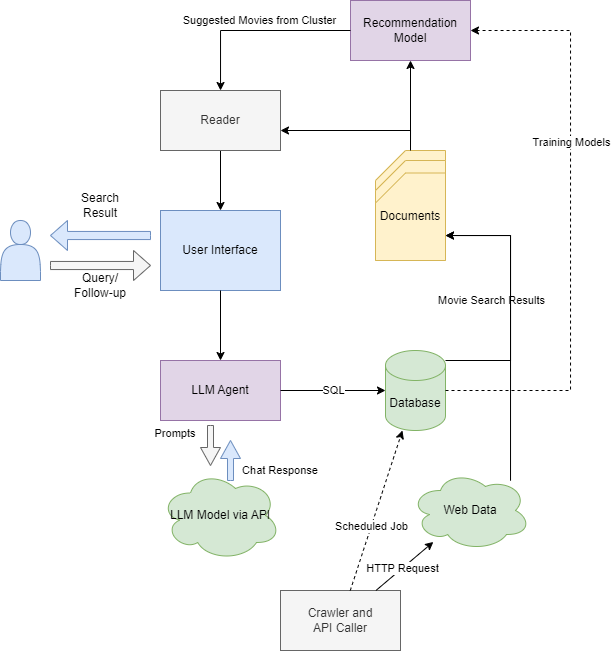
\includegraphics[width=1\linewidth]{doc//report//assets/sysarch_final.png}
    \caption{System Architecture}
    \label{fig:sysarch}
\end{figure}

\begin{enumerate}
    \item  {User Interface}: The user interface consists of a search box for the user to type queries and an area to display search results (response). Most of the major front-end web development frameworks can provide the components we need. It is proposed that we use HTML + CSS + JavaScript as the project’s UI solution. Additional libraries and dependencies may be introduced in the engineering process.

    \item {LLM Agent}: The LLM Agent processes user input through three main tasks. Initially, it combines preamble and user input to construct prompts. If a context exists, it appends the new input to the existing context rather than starting anew. Next, it parses the results to extract a list of titles, preparing for database access in the subsequent step. Finally, it sends the retrieved titles to the recommendation model to obtain clustering results and constructs SQL queries based on both LLM and recommendation results. These queries map to the corresponding movie objects in the database.

    \item {LLM Model via API}: Nearly all LLM via API host provide Python SDK for developers to easily request access to API. Our LLM provider combines Pydantic which allows future integration of requesting specific data structure from LLM.

    \item {Recommendation Model}: The input of the recommendation model is a particular movie entry, top-ranked item of LLM results for instance. It returns other similar movie entries based on the K-Means clustering algorithm. There are other potential methods to recommend movies, such as by returning movie that has the best cosine similarity score in vector model. Further discussion and experiment will follow in the report.

    \item {Reader}: Reader is a component where we gather all the relevant movie entries together and filter the repetitive entries. It provides a list view for user to explore.

    \item {Crawler and API Integration}: The crawler and API caller is responsible for the maintenance of our database. We put new movies on a regular basis into the existing database. External resources such as TMDB API is used to create consistent and smooth user experience.

    \item {Database}: The database serves multiple purposes in the project. For LLM information retrieval, it provides structured movie data to enhance LLM outputs. In training clustering models, the database supplies datasets for both analysis and training purposes.
\end{enumerate}


\section{Approaches}
\subsection{Data and Storage}
The following is the necessary aspects of our approaches to data and storage as well as API integrating.

\subsubsection{Dataset}
The dataset used in the project is expected to include meta information about a movie, such as title, cast and genres. The metadata information will support the data retrieval function using query-document relevance algorithms. The dataset chosen for the project is \textbf{IMDb Non-Commercial Dataset}. The IMDb Non-Commercial Datasets offer subsets of IMDb's extensive data for personal and non-commercial use, with daily refreshes. This data is in tab-separated values (TSV) format with UTF-8 encoding. Each file begins with headers, using '\N' to indicate missing or null fields. Content include titles, their regional variations, basic metadata, crew details, episode information, principal cast and crew roles, and ratings, alongside basic information about individuals in the database. There are more than 1 million observations and 10 columns in the original dataset. Data prepossessing filtered out the non-English movies and movies that are too old. To insure scalability and usability of the system, we remained a majority of the observations and use popularity, the number of movie reviews, to control the corpus size. TSV files are processed by the means of Pandas and then inserted into relational database. The dataset was stripped of any missing values and irrelevant columns. 

\subsubsection{Dataset Used for Model Training}
\textbf{MovieLens} dataset provides another dimension of movie data. For LLM training and performance measuring purpose, ground truth of movie suggestions need to be set. Due to the subjective nature of judging whether movie falls into a category of taste, a large number of samples in categorizing movie data are required. MovieLens is a widely recognized source with extensive metadata on movies. This dataset will provide a foundational source of data for the project, providing user rated tags with a sample size of 15.58M. Figure \ref{fig:ml-tag} shows a 0.1\% of the data distribution. Tags with relavance lower than 0.5 are not considered related to that movie.

\begin{figure}
    \centering
    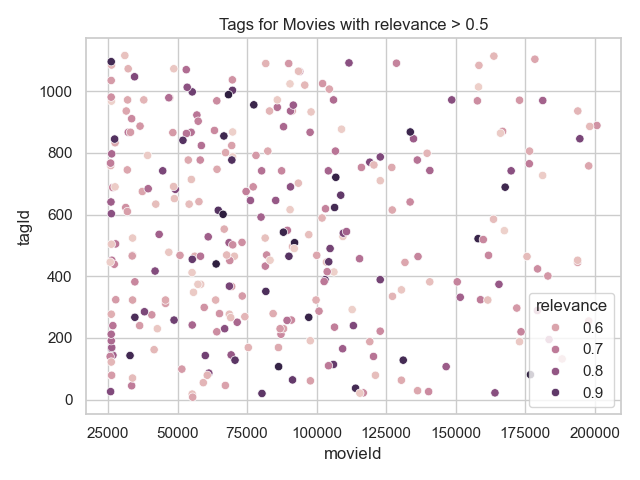
\includegraphics[width=1\linewidth]{doc//report//assets/tags_for_movies.png}
    \caption{Preview of MovieLens Dataset to Link Movies with Tags}
    \label{fig:ml-tag}
\end{figure}

\subsubsection{Database}
The entity relationship diagram in Figure \ref{fig:erd}, visualizes the database structure for the local data storage in our project. It details the "Movie" entity as the core, which includes attributes like movie ID, title, and release date. It is connected to "Actors" and "Directors" through associative entities "MovieActors" and "MovieDirectors," signifying many-to-many relationships, as a movie can have multiple actors and possibly multiple directors, and vice versa. There's also a "MovieGenres" associative entity that links movies to various "Genres," enabling films to be categorized into different genres, reflecting the possibility of a movie belonging to more than one genre. The data present in the database is from imdb’s open datasets\cite{IMDb}. 

\begin{figure}
    \centering
    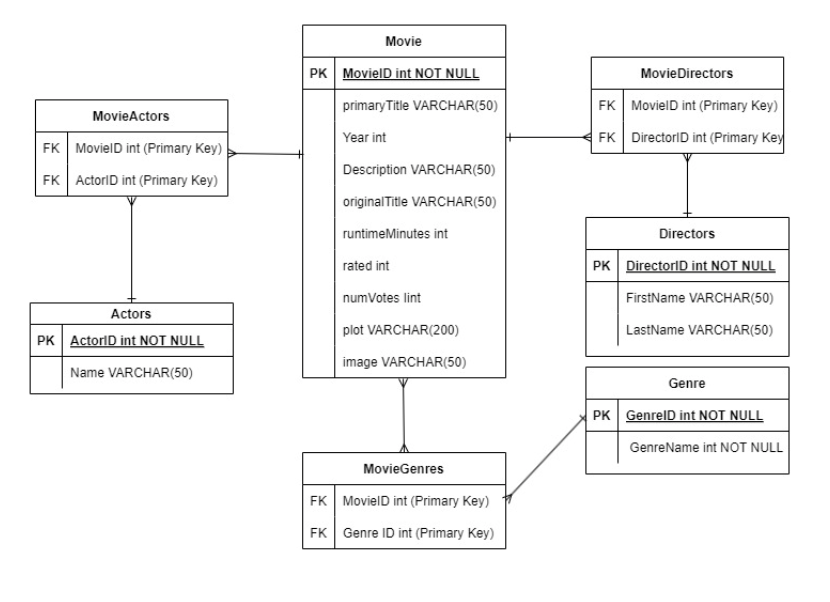
\includegraphics[width=1\linewidth]{doc//report//assets/erd.png}
    \caption{Entity Relationship Diagram}
    \label{fig:erd}
\end{figure}

\subsubsection{Updating Database}
The database is updated every 2 weeks after initial setup. The task of updating database is to download IMDb's new dataset and extract new entries. After filtering and API call, the database is considered synced with the new information.

\subsubsection{API Integrating}
The function of the API and Web Crawler is to provide our system with a substantial amount of data so our system can create and carry out recommendations and search queries. These search queries would be based on the user’s input and then the program will make the accurate call to the APIs used in this project. To enhance the text-based movie metadata, we made use of a third party service, TMDB API. Using the movie ID, which is the \texttt{imdb\_id}, we can send API calls to TMDB to retrieve the description of the movie. This is a piece of string typed information within 100 words for each movie. 

\subsection{Large Language Model}
The proposed Large Language Model for use in this project is based on the Cohere platform. As described in \textbf{Definition III.9}, LLM's response is a string which can be parsed into desired data type. In the testing phase, we also used LLMs to generate test cases and test prompts.

\subsubsection{Model Properties}
The Cohere platform provided the state-of-the-art closed source models for developer to use. The model we used is the general model of the company, which is trained on corpus including a 4.8k movie dataset including plots and cast crew.\cite{cohere_movies_dataset} Cohere LLM showed best results when dealing with movie generating task compare4d with other open source models. During our LLM performance evaluating phase, \texttt{vicuna-7b-v1.5}, which is an open-source chat assistant trained by fine-tuning Llama 2 on user-shared conversations collected from ShareGPT, outperformed the other LLMs, such as LLaMA and ALpaca, of the same scale\cite{zheng2023judging}. This open source model is available and can be downloaded at Hugging Face.  

\subsubsection{LLM Task Design}
\begin{itemize}
  \item \texttt{preamble}: The content included in the preamble are: Interactions are exclusively centered on movies; Focus discussions exclusively on movies; Every response starts with \textit{Welcome to MovieSearch}; When referencing movies, use the format \texttt{<<Name (Year)>>}.
  \item \texttt{prompt}: User Input.
  \item \texttt{chat\_history}: The interactions between user and model of this session. This can be cleared at user's wish.
\end{itemize}

We use Cohere's API for all responses. However, it's not enough to only retrieve text response. More actions will be taken to process the response.

\subsubsection{Model Performance Improvement}
Although LLMs are ideal for fuzzy match, tip-of-the-tongue tasks, there are occasions where LLMs show limited capabilities.

\begin{itemize}
    \item \texttt{Fine-tuning}: Fine-tuning the model using ground truth of movie recommendation helps the generic suggestion questions.

    \item \texttt{Structured Response}: Pydantic is a data validation and settings management library using Python type annotations. Instead of using preamble and regular expression to reformat response, pydantic provides a much faster and accurate response.

    \item \texttt{Outdated Corpus}: Models are not able to provide any information after its latest update. For instance, the model can not provide any description of a movie that is released later than the latest update of the LLM. 
\end{itemize}

% Our team believes that the model is able to provide a decent description even with little prompting and it reaches our expectations. However, there are still two potential issues with the model: 1, we notice that the description of the movie “Saw” in the Fig. \ref{fig:llm} is much shorter than the other three movies. It is not clear why it happens, further tests and prompting may be needed to generate a longer and more detailed description. 2. Due to the nature of the model, it is not able to provide any information after its latest update. In this case, the model can not provide any description of a movie that is released later than the latest update of the LLM. 

\subsection{Recommendation System}
\begin{itemize}
    \item \texttt{Dataset}: The dataset chosen for clustering is extracted from the existing database. It includes the movie release year, genre and plot for clustering.

    \item \texttt{Principle Component Analysis}: There are 24 unique genre categories for all of the movie, making the total number of column to be 31. We leveraged Principle Component Analysis to identify principle component of the dataset. Figure \ref{fig:pca} shows the cumulative explained variance. By obtaining only half of the feature, we can achieve 70\% of total variance, thus improve performance in model training.

    \item \texttt{Genre Clustering}: We used DBSCAN to determine the number of clusters and then K-means to cluster all the movie entries. The features taken into account here are mainly genres.

    \item \texttt{NLP Clustering}: This method only uses one feature, which is a text string of natural language description of movie. We first removed punctuation, stop words from dataset, then used Lemmatization to stem the words, finally we utilized \texttt{TfidfVectorizer} from \texttt{scikit-learn} to vectorize data and calculate TF-IDF values.
    


\end{itemize}
We compared two methods to recommend movies. After evaluating performance on ground truth dataset based on sequential movies, we found that NLP clustering achieved better results, although taking longer time to train and feed forward. The downside of TF-IDF based method is that it takes significantly longer than the other one.

\begin{figure}
    \centering
    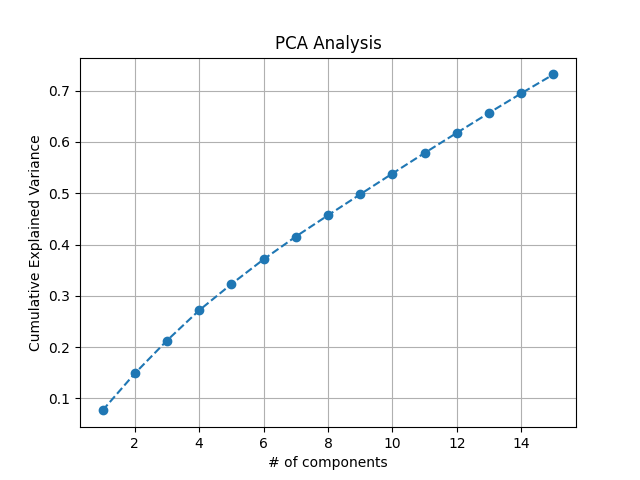
\includegraphics[width=1\linewidth]{doc//report//assets/pca_analysis.png}
    \caption{Principle Component Analysis}
    \label{fig:pca}
\end{figure}


\subsection{User Interface}
The user interface is an application that allows the user to write queries based on their needs. The application will then implement the methods explained earlier, and provide users with exact results, and recommendations.

\subsection{REST API}
This section explains the REST API created for and used in this project. The REST API provides our back end and fronted with the information necessary in this project. The following list is each endpoint or route implemented and used within the project.
\begin{itemize}
  \item \texttt{/movies/}
  \item \texttt{/directors/}
  \item \texttt{/listofmovies/}
  \item \texttt{/search/}
\end{itemize}

Each of the return values from the previous list are in JSON format. The\texttt{ /movies/} takes a unique identifier for a movie, and returns to our program all meta-data of that movie. This meta data is consistent with the view page of our application. The view page is explained in more depth in a later section. The \texttt{/directors} endpoint, when given a unique identifier of a director returns the name of a director. The \texttt{/listofmovies/} is a POST method that takes in a list of movies as a parameter. The \texttt{/search/} takes in a query as a parameter and returns movies that have a plot or title that is the most similar to the query.

% \begin{figure}
%     \centering
%     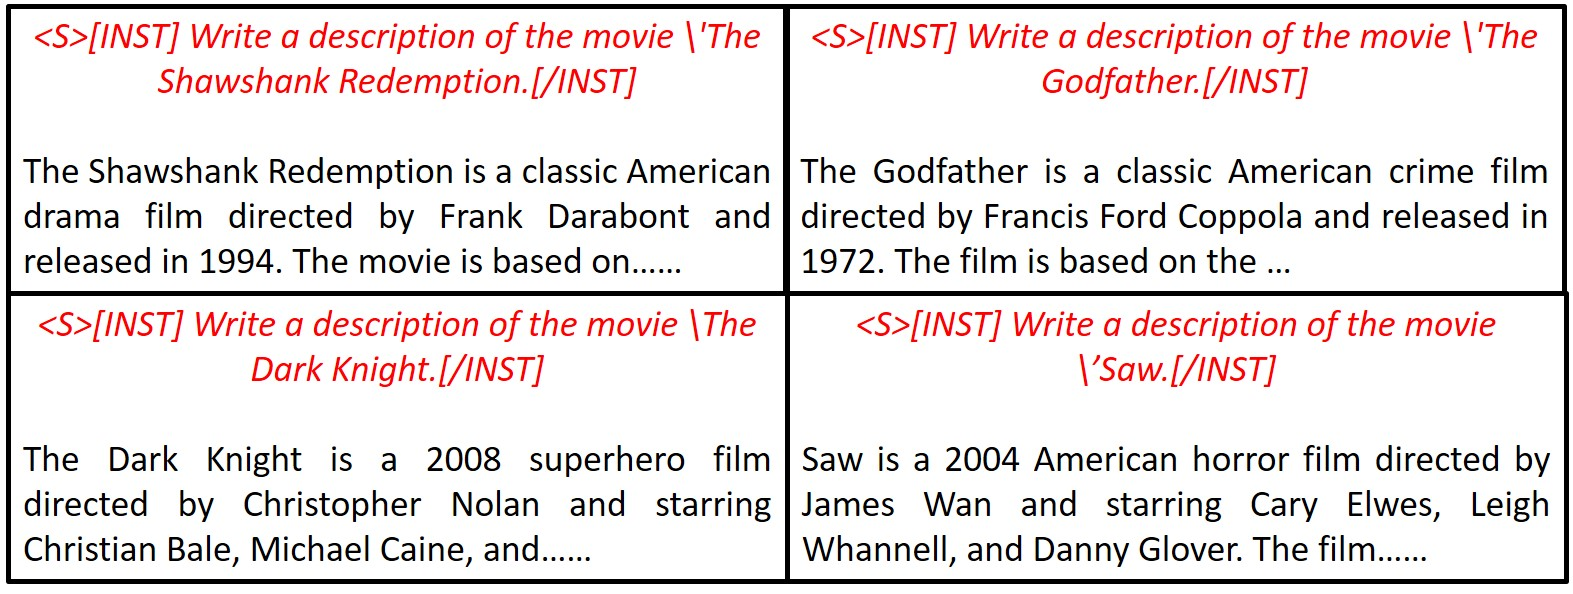
\includegraphics[width=1\linewidth]{doc//report//assets/llmresults.jpg}
%     \caption{The input (the red and italics context at the top) and output (the black context) of the large language model. The full output of each movie test can be found in the appendix
% }
%     \label{fig:llm}
% \end{figure}


\section{Implementation}
%User interface Section
\subsection{User Interface}
This section explains the user interface (UI). The UI of our project serves as the only means for users to interact with the system. It is designed to be intuitive and user-friendly, facilitating seamless communication between the user and the back-end.



\subsubsection{Technologies Used}
The front end implementation was created using following and how it's used in our project.
\begin{itemize}
  \item \textbf{HTML:} Creates the Structure and components used. 
  \item \textbf{CSS:} Styles the web page, so its not default HTML.
  \item \textbf{Java Script:} Dynamically updates the web page based on condition.
\end{itemize}

\subsubsection{Default Home Page}
The image in Figure \ref{fig:default} shows the initial view users encounter upon opening the web page. This interface prominently features a search bar and a "Clear Memory" button. The "Clear Memory" button allows users to erase their chat history, ensuring that the LLM does not remember previous queries. However in this state there is not any chat history to be cleared.

\begin{figure}
    \centering
    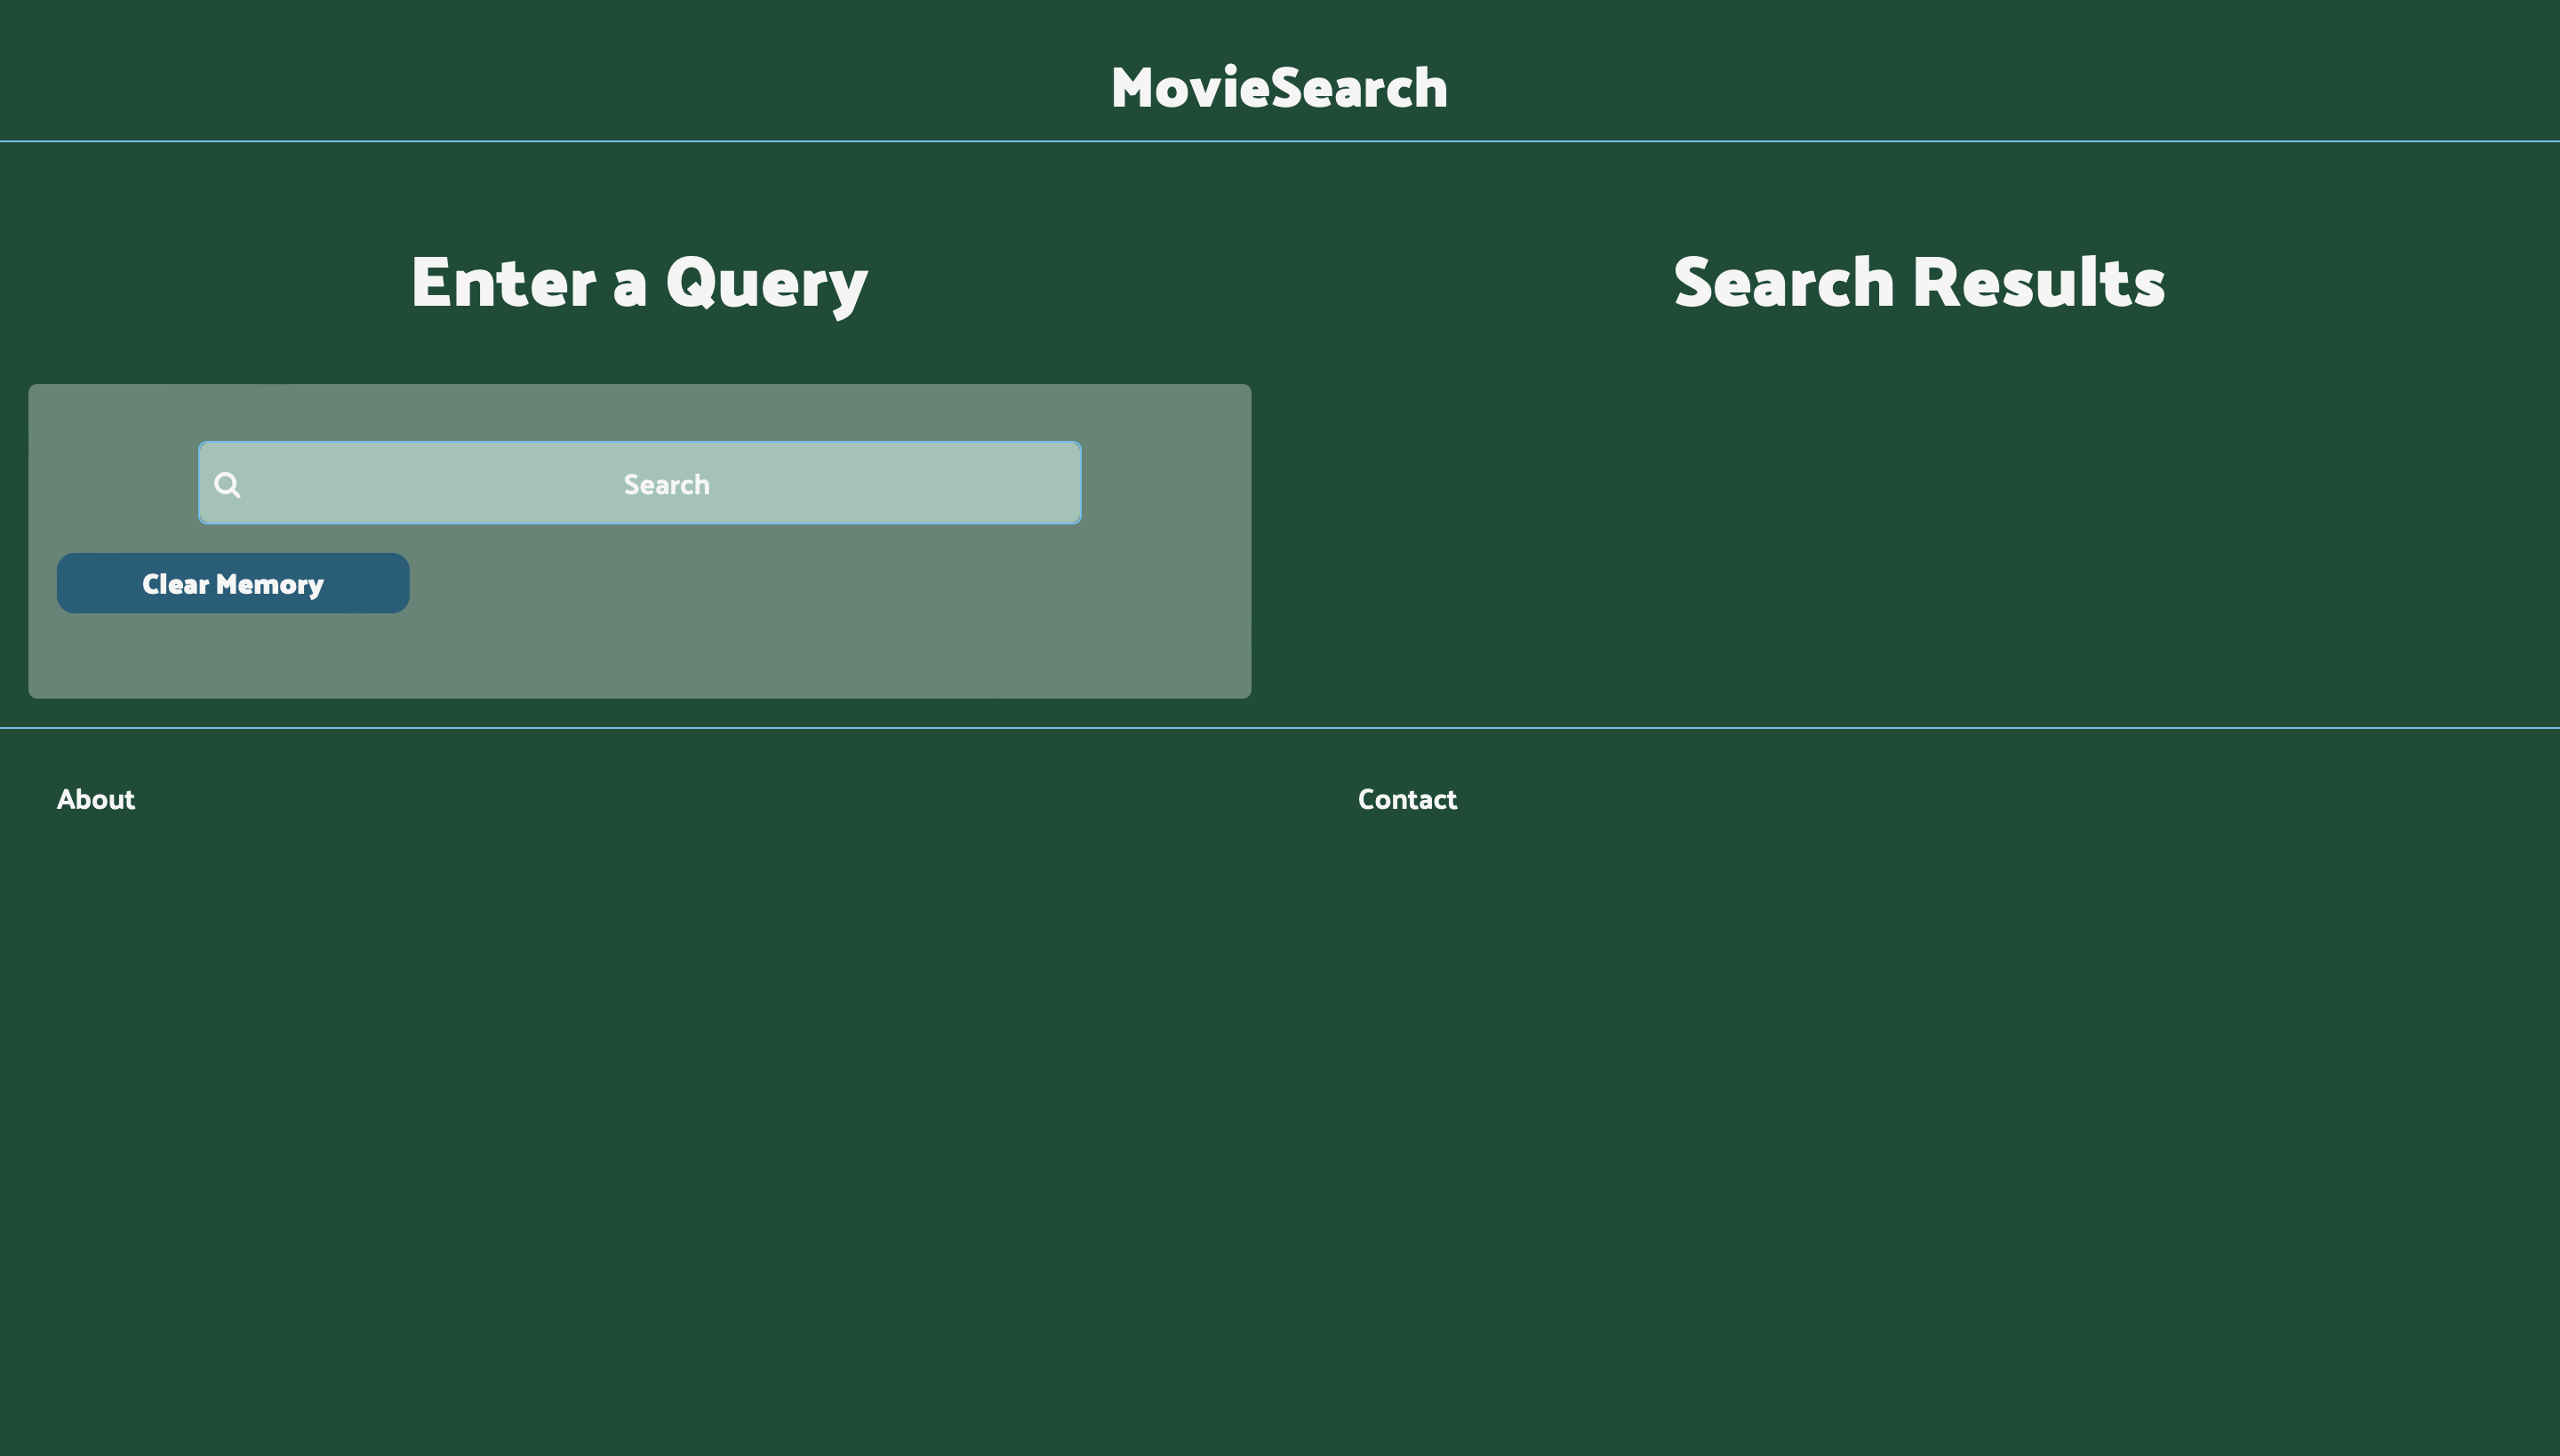
\includegraphics[width=1\linewidth]{doc//report//assets/Defaullt.png}
    \caption{Default User Interface Screenshot}
    \label{fig:default}
\end{figure}

\subsubsection{Left Side (Chat/Search Interface)}
The image in Figure \ref{fig:results} is a screenshot of the user interface demonstrating an example of what the UI looks like after a search has been made. The left side features an interface like a chat messenger. This is where users can input queries such as asking for movie suggestions based on specific criteria or genres, or searching for movies by name.  The queries are submitted by clicking upon the search icon or pressing \texttt{Enter/Return} on a keyboard. Above the search bar, there's an area that displays the ongoing conversation between the user and the responses from the Large Language Model. Whenever the LLM responds to a user's query, the response is typed out on the screen as if it is typing a response in real-time. The query in Figure \ref{fig:results} has a formatted output. The LLM provides a response in the format of: \textless\textless \texttt{MovieName Year}\textgreater\textgreater. If the response contains multiple movies its format is: \texttt{-}\textless\textless \texttt{MovieName Year}\textgreater\textgreater. The \texttt{-} lets Java Script know to format the movies as a list. 

\begin{figure}
    \centering
    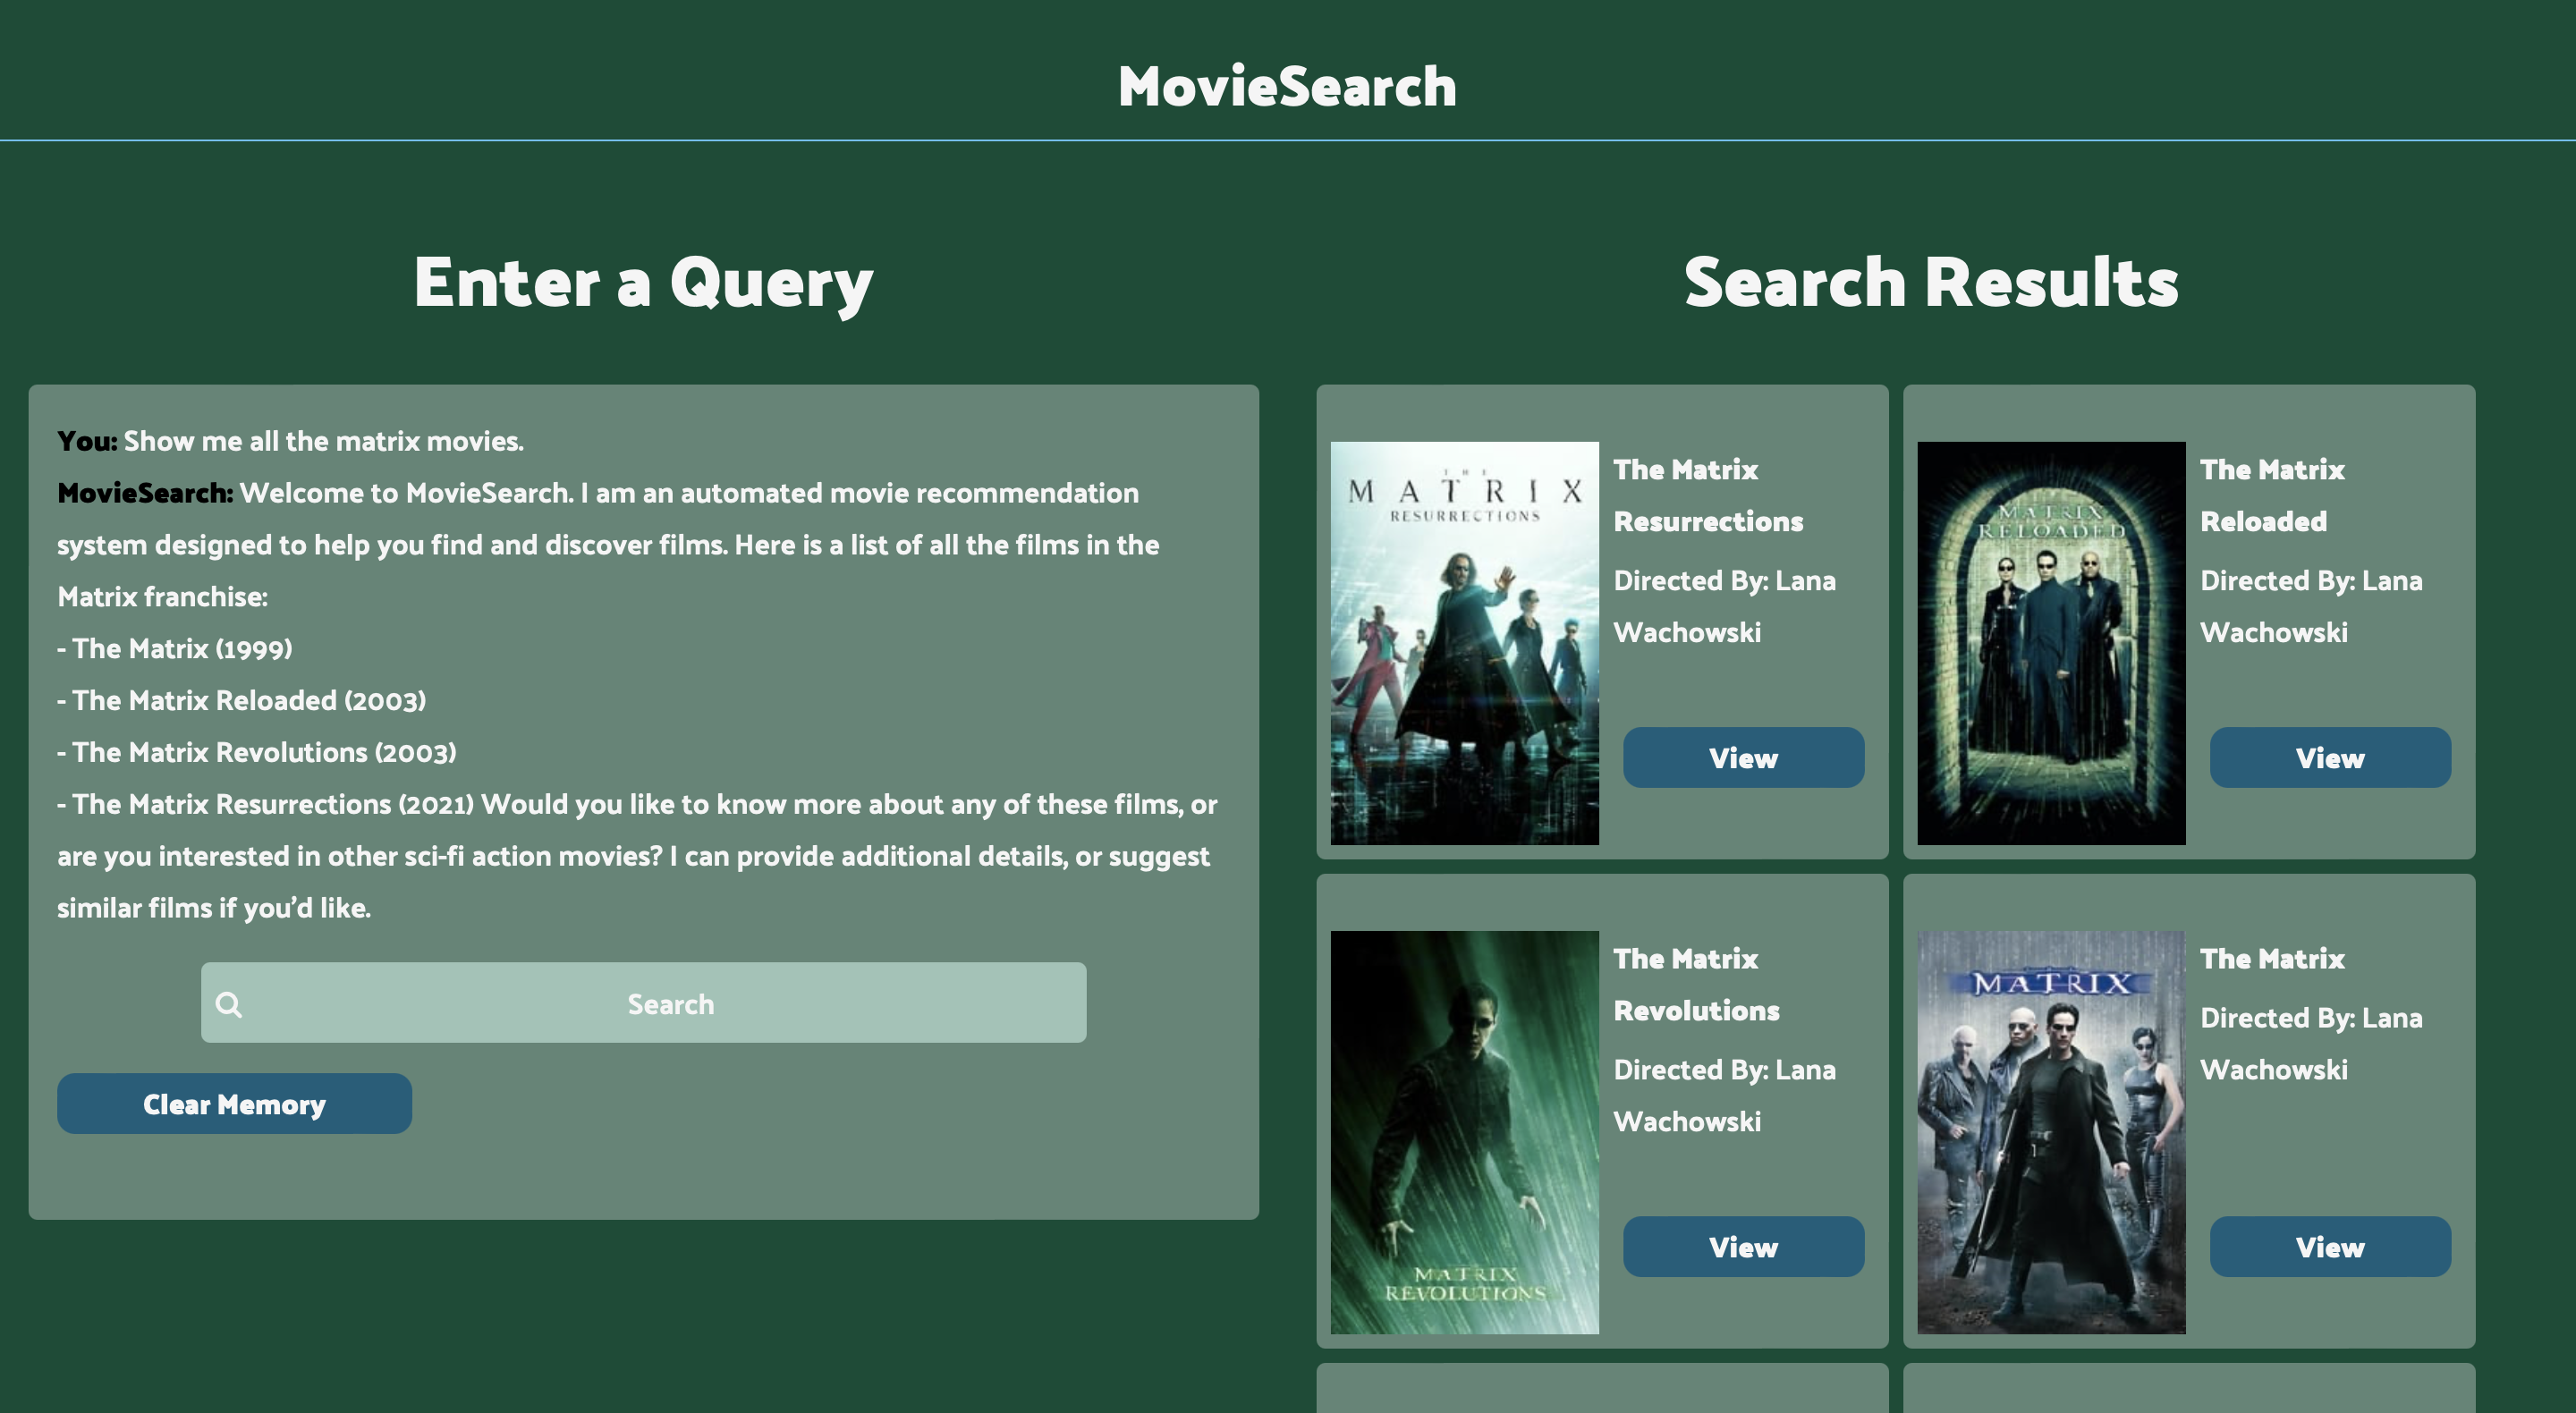
\includegraphics[width=1\linewidth]{doc//report//assets/Results.png}
    \caption{LLM Response User Interface Screenshot}
    \label{fig:results}
\end{figure}

\subsubsection{Right Side (Search Results)}
On the right side of Figure \ref{fig:results}, there is a 'Search Results' area that showcases the movies mentioned in our LLM's response. Each movie is displayed with a visual representation (like a movie poster), the name of the movie, and the director's name. To see additional information users can click the 'View' button, this page is explained in the next section. Depending on the results of the users query the search results are updated dynamically. There are two conditions where the results don't change when the chat changes. One condition is when the user clicks clear memory. The other condition is when a query doesn't yield any results.

\subsubsection{View Page}
Figure \ref{fig:view} shows an individual result. This page is only accessible after a user clicks the view button present in Figure \ref{fig:results}. This page contains more in depth data of a particular movie. The information presented is, Movie title, year, plot, director(s), and actors located at the bottom of the page.

\begin{figure}
    \centering
    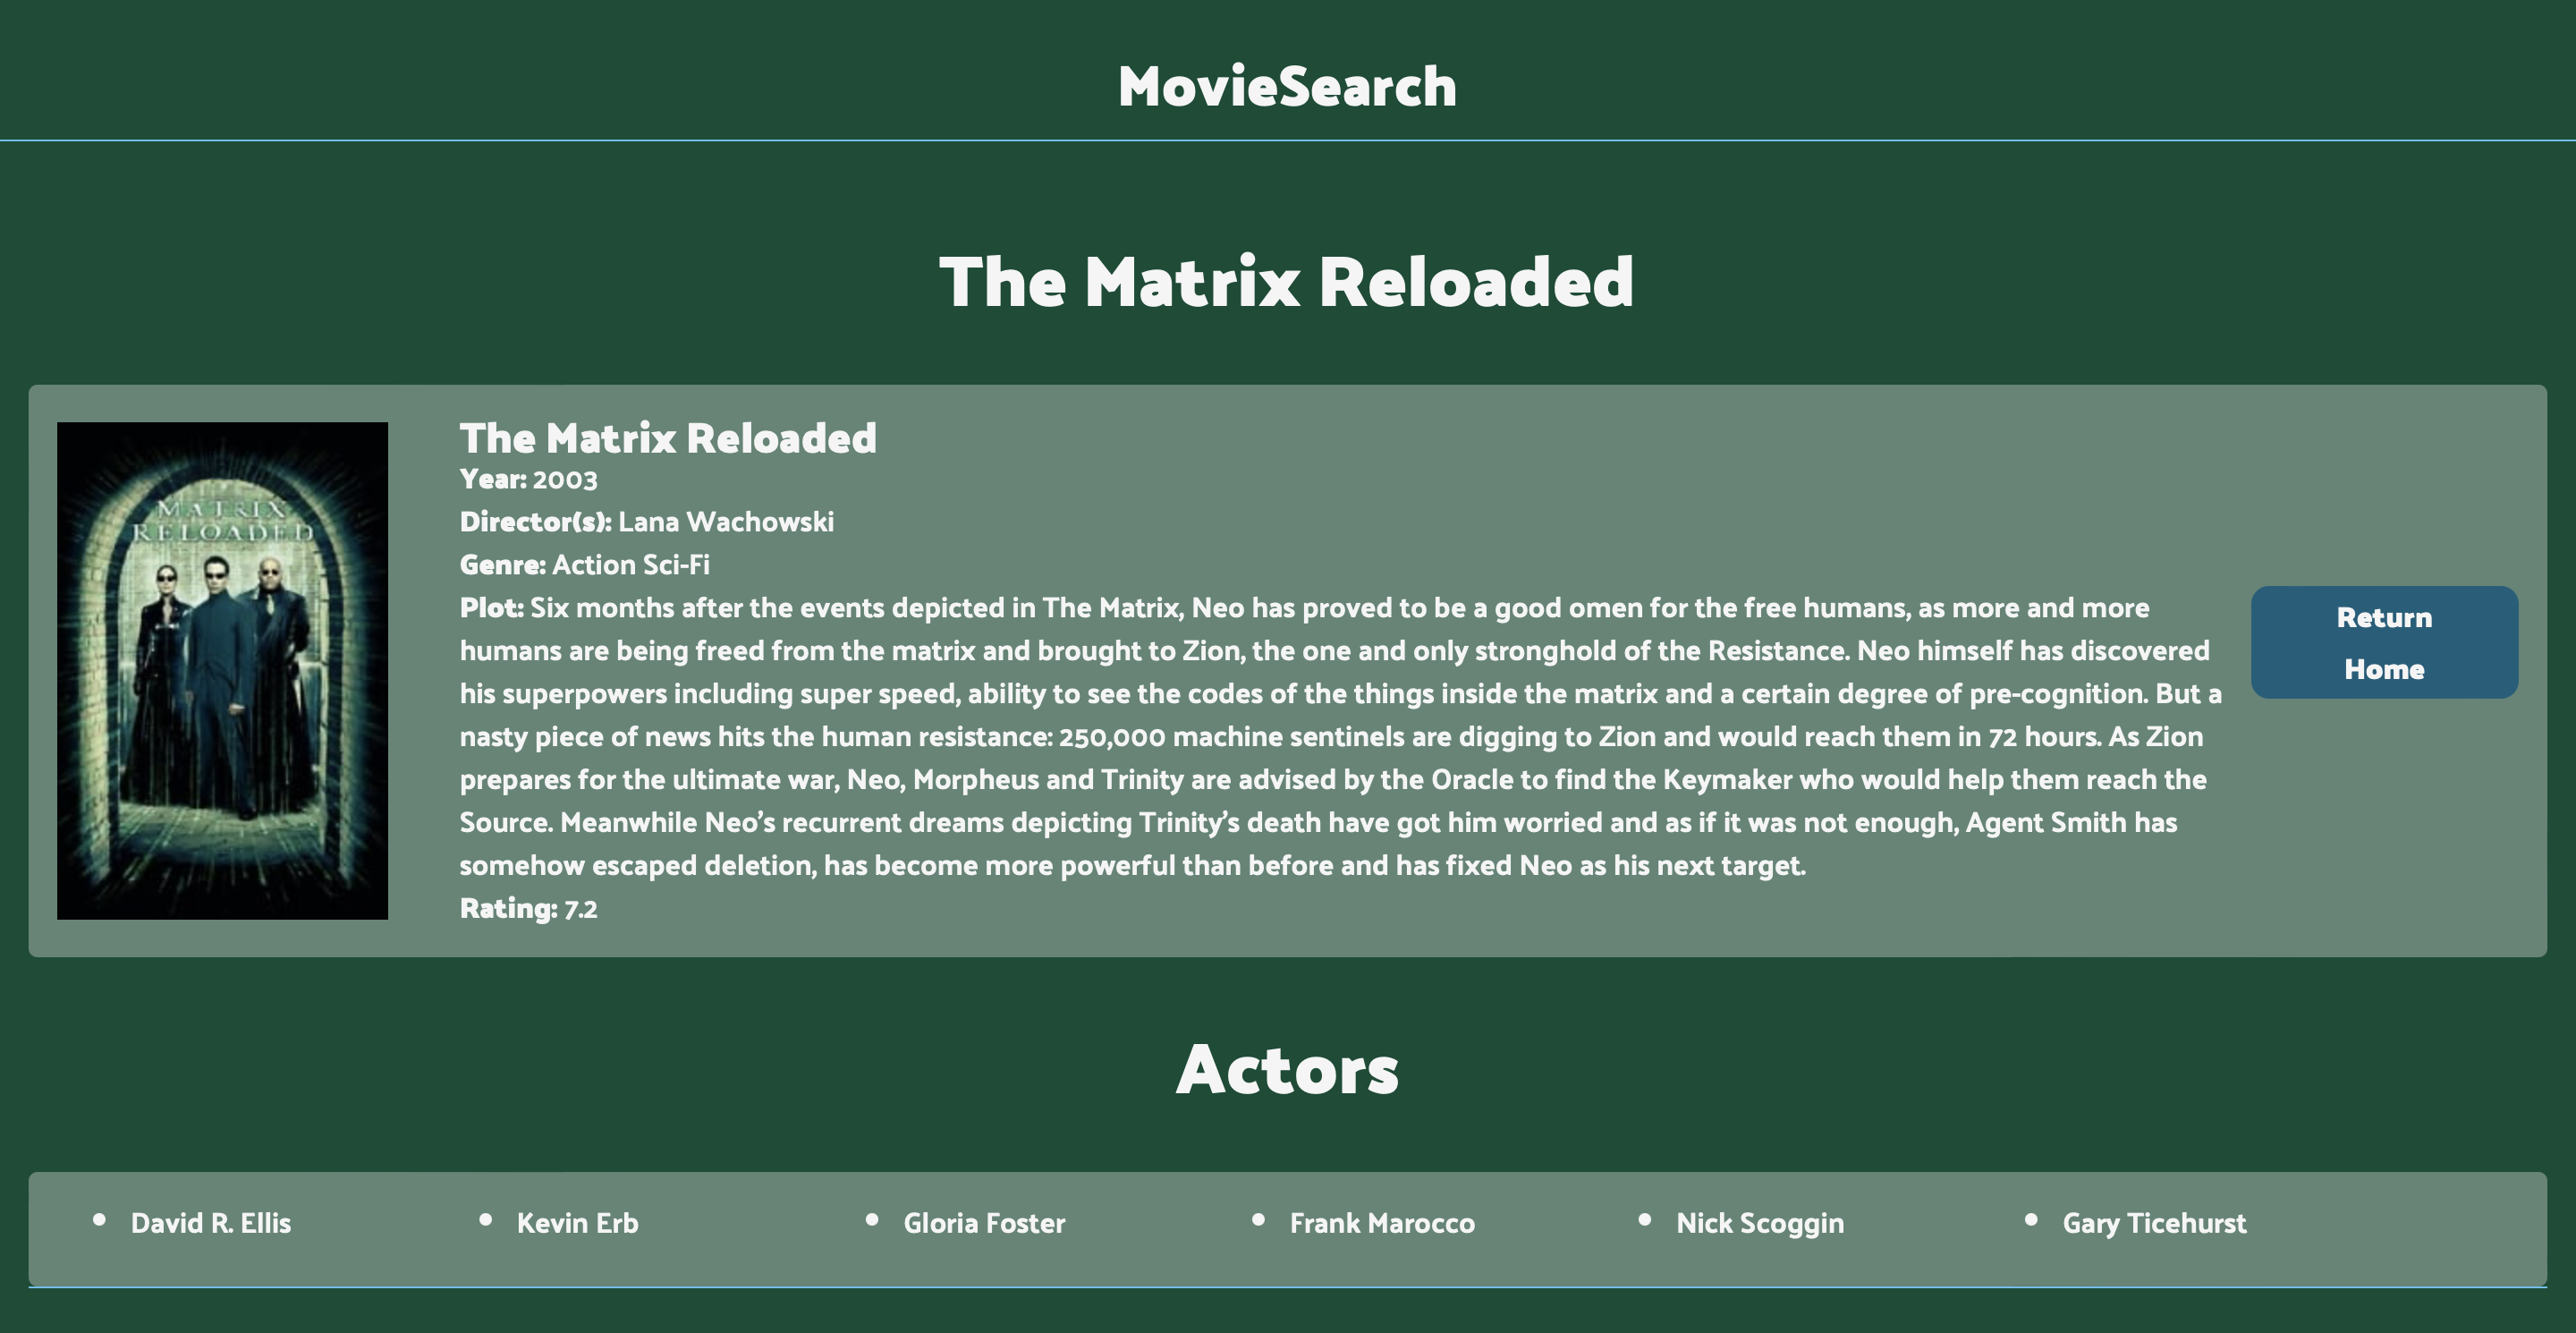
\includegraphics[width=1\linewidth]{doc//report//assets/view.png}
    \caption{View Page User Interface Screenshot}
    \label{fig:view}
\end{figure}



%User interface Section
\subsection{Server}
\subsubsection{Database Server}
The data server is built using FastAPI. The purpose of the server is to provide fast response to users' query. Based on the questions defined in Design Overview, a versatile as well as Machine Learning supportive environment is required. Hence we use Python and its development ecosystems. Developer compared Django and FastAPI as the back-end service framework. Django provides thorough support for data modeling and API design, but it is not light-weighted. The admin and authorization built-in methods are not needed and it requires manual checking in modeling for legacy database, which introduces risks. FastAPI, however, provides high-performance and low-dependency server solution for the project. To interact with the relational database, we leveraged \texttt{sqlalchemy} and \texttt{pydantic} as the solution for Object Relational Mapper (ORM) solution. Table \ref{tab:data_server} shows the logging massage of dataserver

\vspace{10}
\begin{table}[ht]
\centering
\scriptsize
\caption{Data Server Sample Output}
\label{tab:data_server}
\begin{tabular}{>{\ttfamily}l >{\ttfamily}l}
\hline
INFO:     & Application startup complete. \\
INFO: & Movies: [ \\
          & <models.Movie object at 0x1078b13f0>, \\
          & <models.Movie object at 0x10790bb80>, \\
          & <models.Movie object at 0x10790bbe0>, \\
          & ...
          & ] \\
INFO:     & X.X.X.X - "POST /listofmovies/ HTTP/1.1" 200 OK \\
\hline
\end{tabular}
\end{table}
\vspace{10}


\subsubsection{ORM Models} 

Utilizing a pre-existing database, the main task in the ORM modeling is to map the Python objects to the data field to the table. To maintain the relationship of entities, we added \texttt{back\_populates} feature of \texttt{sqlalchemy} to properly describe the many-to-many relationship. When retrieved data from table, we used \texttt{pydantic} to transfer the data into object in response.

\subsubsection{Response Building} 
The server interacts with user interface using RESTful API. An API endpoint with GET method is implemented to achieve the goal. The API returns mapped movie objects as a JSON string in the response body.

\subsubsection{Application Server}
The application server is built using Flask. The purpose of the server is to host user interface, LLM agent and retrieve results from data server. To accompany classical machine learning model backed recommendation system, the application server loads the model and dataset for smooth mapping and clustering. Table \ref{tab:app_server} shows results retrieved in different phases in Flask server.


\begin{table}[ht]
\centering
\scriptsize
\caption{Application Server Sample Output}
\label{tab:app_server}
\begin{tabular}{|m{1.2cm}|p{5.8cm}|}
\hline
\texttt{LLM} & \texttt{['The Matrix (1999)', 'The Matrix Reloaded (2003)', 'The Matrix Revolutions (2003)', 'The Matrix Resurrections (2021)', 'The Matrix (1999)']} \\
\texttt{Rec.} & \texttt{['The Avengers (2012)', 'Captain America: Civil War (2016)', 'Iron Man 2 (2010)', 'X-Men: First Class (2011)', 'The Matrix Reloaded (2003)', 'The Matrix Revolutions (2003)', 'X-Men Origins: Wolverine (2009)', 'The Wolverine (2013)', 'Face/Off (1997)']} \\
\texttt{Results} & \texttt{['The Matrix (1999)', 'The Matrix Reloaded (2003)', 'The Matrix Revolutions (2003)', 'The Matrix Resurrections (2021)', 'The Avengers (2012)', 'Captain America: Civil War (2016)', 'Iron Man 2 (2010)', 'X-Men: First Class (2011)', 'X-Men Origins: Wolverine (2009)', 'The Wolverine (2013)', 'Face/Off (1997)']} \\
\hline
\end{tabular}
\end{table}
\vspace{10}

\subsection{Large Language Model}
\subsubsection{Genre Searching: }  Table \ref{tab:genre} shows an example of how LLM response to general genre searching.

\vspace{10}
\begin{table}[ht]
\centering
\scriptsize
\caption{Genre Searching Sample Output}
\label{tab:genre}
\begin{tabular}{|p{0.5cm}|p{6.5cm}|}
\hline
\texttt{User} & \texttt{funny movie} \\
\texttt{LLM} & \texttt{'Welcome to MovieSearch. I am an automated movie recommendation system designed to help you find the perfect film for your mood. \n\nThere are many hilarious movies that can brighten your day and bring a smile to your face. Here are a few popular choices: \n\n- <<The Hangover (2009)>>: This raunchy comedy follows a group of friends as they try to piece together a wild bachelor party in Las Vegas and find their missing groom. \n\n- <<Bridesmaids (2011)>>: ... (introduction) \n\n- <<Superbad (2007)>>: ... \n\n- <<Anchorman: The Legend of Ron Burgundy (2004)>>: ... \n\n- <<21 Jump Street (2012)>>: .... \n\nIf '}] \\
\hline
\end{tabular}
\end{table}
\vspace{10}

\subsubsection{Tip-of-the-tongue Searching: }  Table \ref{tab:tott} shows an example of how LLM response to Tip-of-the-tongue searching scenarios. User only needs to briefly mention a part of the plot in the movie and LLM will match to the most possible movie which contains the information.

\vspace{10}
\begin{table}[ht]
\centering
\scriptsize
\caption{TOTT Sample Output}
\label{tab:tott}
\begin{tabular}{|p{0.5cm}|p{6.5cm}|}
\hline
\texttt{User} & \texttt{a man run across the united states} \\
\texttt{LLM} & \texttt{'Welcome to MovieSearch. \n\nI think you may be referring to the movie <<\textbf{Forrest Gump (1994)}>>. In this film, the titular character, played by Tom Hanks, embarks on a cross-country run multiple times throughout his life. The movie is a heartwarming and humorous tale that has become a classic. \n\nIf this doesn't match what you're looking for, could you provide some more details or keywords to help narrow down the search? Alternatively, I can suggest some similar movies about journeys across America, such as <<Zombieland (2009)>>, <<Little Miss Sunshine (2006)>>, or <<Easy Rider (1969)>>.'}] \\
\hline
\end{tabular}
\end{table}
\vspace{10}

\subsubsection{Personalized Searching: }  Table \ref{tab:personalized} shows how a large language model responds to personalized search scenarios. In such instances, users might share details about their mood, surroundings, and specific occasions, prompting the model to offer tailored suggestions based on the provided information. The LLM asks back to user to provide more specific information.

\vspace{10}
\begin{table}[ht]
\centering
\scriptsize
\caption{Personalized Recommendation Sample Output}
\label{tab:personalized}
\begin{tabular}{|p{0.5cm}|p{6.5cm}|}
\hline
\texttt{User} & \texttt{i invited some of my friends home for a party, what should we watch} \\
\texttt{LLM} & \texttt{'Welcome to MovieSearch. I'd be happy to help you find a movie for your party! \textbf{Could you give me some more details about the kind of movies your friends enjoy?} With a few more details, I can provide some great suggestions! \n\nIn the meantime, here are a few crowd-pleasers that might be worth considering: \n\n- <<The Hangover (2009)>>: ... \n\n- <<Avengers: Endgame (2019)>>: ... \n\n- <<The Wolf of Wall Street (2013)>>: ... \n\n- <<The Greatest Showman (2017)>>: ... \n\nLet me know if any of these spark your interest, or if you'd like me to suggest something else based on your friends' tastes! '}] \\
\hline
\end{tabular}
\end{table}
\vspace{10}

\subsection{Recommendation Model}
\subsubsection{Clustering based on genre} To determine cluster size, we used DBSCAN algorithm. We used PCA transformed dataset (Component: 15, Variance: 70\%) for DBSCAN training, and based on 0.3 eps, the recommended number of clusters is 286.

\bigskip
\begin{center} % Start the center environment
\begin{tabular}{l| r}
    Metrics & Value \\
    \hline
    \texttt{\# of Cluster} & \texttt{286} \\  
    \texttt{\# of Noise Points} & \texttt{3334} \\
\end{tabular}
\end{center} % End the center environment
\bigskip

We created K-means model with a cluster size of 286. After LLM responded with movie titles, we find the entry in the dataset and retrieve the cluster label. Because typically there are hundreds of movies in one cluster label, we rank the results based on their popularity \( P \), following the equation below.
\[ P = N \cdot r\] where $N$ is the number of votes and $r$ is the average rating. This approach focus more on the popular titles.

\subsubsection{Clustering based on plot} TF-IDF matrix is applied to find out the similarity of two movies' description. We utilized \texttt{nltk} to pre-process the plain text. Punctuation and stop words are removed, words are stemmed using Lemmatization. Table \ref{tab:preprocess} shows the difference before and after pre-processing for movie \textit{Forrest Gump (1994)}.


\begin{table}[h]
\centering
\caption{Text Pre-processing Example}
\label{tab:preprocess}
\begin{tabular}{|>{\centering\arraybackslash}m{3.5cm}|>{\centering\arraybackslash}m{3.5cm}|}
\hline
\textbf{Before} & \textbf{After} \\
\hline
A man with a low IQ has accomplished great things in his life and been present during significant historic events—in each case, far exceeding what anyone imagined he could do. But despite all he has achieved, his one true love eludes him. & man low iq accomplish great thing life present significant historic case far exceed anyone imagine could despite achieve one true love elude \\
\hline
\end{tabular}
\end{table}

% \begin{table}[h]
% \centering
% \caption{Text Pre-processing Example}
% \label{tab:preprocess}
% \begin{tabular}{|>{\centering\arraybackslash}p{3.5cm}|>{\centering\arraybackslash}p{3.5cm}|}
% \hline
% \textbf{Before} & \textbf{After} \\
% \hline
% A man with a low IQ has accomplished great things in his life and been present during significant historic events—in each case, far exceeding what anyone imagined he could do. But despite all he has achieved, his one true love eludes him. & man low iq accomplish great thing life present significant historic case far exceed anyone imagine could despite achieve one true love elude \\
% \hline
% \end{tabular}
% \end{table}

% \begin{table}[h]
% \centering
% \caption{Text Pre-processing Example}
% \label{tab:preprocess}
% \begin{tabular}{|>{\raggedright\arraybackslash}p{3.5cm}|>{\raggedright\arraybackslash}p{3.5cm}|}
% \hline
% \textbf{Before} & \textbf{After} \\
% \hline
% A man with a low IQ has accomplished great things in his life and been present during significant historic events—in each case, far exceeding what anyone imagined he could do. But despite all he has achieved, his one true love eludes him. & man low iq accomplish great thing life present significant historic case far exceed anyone imagine could despite achieve one true love elude \\
% \hline
% \end{tabular}
% \end{table}

After pre-processing, TF-IDF matrix is built using \texttt{TfidfVectorizer} of \texttt{scikit-learn}. The TF-IDF matrix is a $41974 \times 52741$ shaped sparse matrix. There are 41974 movies taken into account in total, and the corpus size is 52741. We calculate the cosine similarity between each movie pairs. Finally, we have a $41974 \times 41974$ shaped similarity matrix that indicates any two movies' similarity.

For a given movie title, we find top 10 movies that have the highest cosine similarity to the given movie, return the titles.

\subsection{Evaluation Metrics}
\subsubsection{Ground Truth for LLM Recommendation} It's difficult to find a ground truth for movie recommendations because of the more free and personalized task we want LLM to handle. Classifying a movie into a category or genre can rely on the initial genre that's predefined for a movie. This often used as training data for LLMs. However, we did not find any training data that can map tags or features like \textit{computer animation}, \textit{good sequel}. To better test LLM's response on more interesting and generalized questions, we construct a ground truth dataset based on tags.

MovieLens provided us with a 25M observation user rating of movies. Of the dataset, there is a table containing the human labeling tags of the movie. Each tag and movie has a relevance score that is in the range \((0, 1)\). We selected the tag-movie pair whose relevance is higher than 0.5, and found all the movies that are related to the tag.

To fairly test the inference performance, we used \texttt{Neural-Chat-7B} to generate questions based on tags. An example of tag and question generated can be found in Table \ref{tab:ground_truth_topic}.

\begin{table}[ht]
\centering
\scriptsize
\caption{Topic Ground Truth}
\label{tab:ground_truth_topic}
\begin{tabular}{|>{\centering\arraybackslash}m{1.5cm}|>{\centering\arraybackslash}m{2.1cm}|>{\centering\arraybackslash}m{3.4cm}|}
\hline
\textbf{Tag} & \textbf{Question} & \textbf{Expected Movies} \\
\hline
\texttt{penguins} & \texttt{'What are some popular movies featuring penguins as main characters or significant roles?'} & \texttt{Madagascar (2005) | March of the Penguins (Marche de l'empereur, La) (2005) | Happy Feet (2006) | Surf's Up (2007) | Madagascar: Escape 2 Africa (2008) ...} \\
\hline
\texttt{poignant} & \texttt{'Can you recommend a poignant movie that touches the heart and evokes strong emotions?'} & \texttt{Léon: The Professional (a.k.a. The Professional) (Léon) (1994) | Shawshank Redemption, The (1994) | To Live (Huozhe) (1994) | What's Eating Gilbert Grape (1993) | Muriel's Wedding (1994) | Forrest Gump (1994) ...} \\
\hline
\texttt{surprisingly clever} & \texttt{'Can you recommend a surprisingly clever movie that might leave a lasting impression?'} & \texttt{Toy Story (1995) | Heat (1995) | Casino (1995) | Twelve Monkeys (a.k.a. 12 Monkeys) (1995) | Seven (a.k.a. Se7en) (1995) ...} \\
\hline
\end{tabular}
\end{table}

% \begin{table}[ht]
% \centering
% \scriptsize
% \caption{Topic Ground Truth}
% \label{tab:ground_truth_topic}
% \begin{tabular}{|p{1.5cm}|p{2.1cm}|p{3.4cm}|}
% \hline
% \textbf{Tag} & \textbf{Question} & \textbf{Expected Movies} \\
% \hline
% \texttt{penguins} & \texttt{'What are some popular movies featuring penguins as main characters or significant roles?'} & \texttt{Madagascar (2005) | March of the Penguins (Marche de l'empereur, La) (2005) | Happy Feet (2006) | Surf's Up (2007) | Madagascar: Escape 2 Africa (2008) ...} \\
% \hline
% \texttt{poignant} & \texttt{'Can you recommend a poignant movie that touches the heart and evokes strong emotions?'} & \texttt{Léon: The Professional (a.k.a. The Professional) (Léon) (1994) | Shawshank Redemption, The (1994) | To Live (Huozhe) (1994) | What's Eating Gilbert Grape (1993) | Muriel's Wedding (1994) | Forrest Gump (1994) ...} \\
% \hline
% \texttt{suprisingly clever} & \texttt{'Can you recommend a surprisingly clever movie that might leave a lasting impression?'} & \texttt{Toy Story (1995) | Heat (1995) | Casino (1995) | Twelve Monkeys (a.k.a. 12 Monkeys) (1995) | Seven (a.k.a. Se7en) (1995) ...} \\
% \hline
% \end{tabular}
% \end{table}


\subsubsection{Ground Truth for Cluster Recommendation} For cluster recommendation, however, it's a even more subjective topic since there's countless view on how movies are similar to each other. To test the performance of clustering, we build a dataset that consists of sequel movies. Since we consider sequels following pattern X: Part 1 and X: Part 2 different movies, and movies in one sequel are more likely to be considered similar on the most scales. An example of this ground truth can be found in Table \ref{tab:similarity_ground_truth}.

\begin{table}[ht]
\centering
\scriptsize
\caption{Similarity Ground Truth}
\label{tab:similarity_ground_truth}
\begin{tabular}{|>{\centering\arraybackslash}m{2cm}|>{\centering\arraybackslash}m{5cm}|}
\hline
\textbf{Movie} & \textbf{Expected Recommendations} \\
\hline
\texttt{Harry Potter and the Sorcerer's Stone (2001)} & \texttt{"Harry Potter and the Chamber of Secrets (2002) | Harry Potter and the Prisoner of Azkaban (2004) | Harry Potter and the Goblet of Fire (2005) | Harry Potter and the Order of the Phoenix (2007) | Harry Potter and the Half-Blood Prince (2009) | Harry Potter and the Deathly Hallows: Part 1 (2010) | Harry Potter and the Deathly Hallows: Part 2 (2011)"} \\
\hline
\texttt{Transformers (2007)} & \texttt{"Transformers: Revenge of the Fallen (2009) | Transformers: Dark of the Moon (2011) | Transformers: Age of Extinction (2014) | Transformers: The Last Knight (2017)"} \\
\hline
\texttt{Jurassic Park (1993)} & \texttt{The Lost World: Jurassic Park (1997) | Jurassic Park III (2001) | Jurassic World (2015) | Jurassic World: Fallen Kingdom (2018) | Jurassic World: Dominion (2022)} \\
\hline
\end{tabular}
\end{table}
% \begin{table}[ht]
% \centering
% \scriptsize
% \caption{Similarity Ground Truth}
% \label{tab:similarity_ground_truth}
% \begin{tabular}{|p{2cm}|p{5cm}|}
% \hline
% \textbf{Movie} & \textbf{Expected Recommendations} \\
% \hline
% \texttt{Harry Potter and the Sorcerer's Stone (2001)} & \texttt{"Harry Potter and the Chamber of Secrets (2002) | Harry Potter and the Prisoner of Azkaban (2004) | Harry Potter and the Goblet of Fire (2005) | Harry Potter and the Order of the Phoenix (2007) | Harry Potter and the Half-Blood Prince (2009) | Harry Potter and the Deathly Hallows: Part 1 (2010) | Harry Potter and the Deathly Hallows: Part 2 (2011)"} \\
% \hline
% \texttt{Transformers (2007)} & \texttt{"Transformers: Revenge of the Fallen (2009) | Transformers: Dark of the Moon (2011) | Transformers: Age of Extinction (2014) | Transformers: The Last Knight (2017)"} \\
% \hline
% \texttt{Jurassic Park (1993)} & \texttt{The Lost World: Jurassic Park (1997) | Jurassic Park III (2001) | Jurassic World (2015) | Jurassic World: Fallen Kingdom (2018) | Jurassic World: Dominion (2022)} \\
% \hline
% \end{tabular}
% \end{table}

\subsubsection{Evaluation Model} For LLM recommendation, a test pipeline is introduced. For each row of the topic ground truth dataset, we build test stub to call the function in app server that's responsible for getting LLM response. We select only the titles parsed by the agent, and compared the current titles with the expected titles in the topic ground truth dataset.

We built a result dataset to record LLM performance during testing phase. An example of the LLM recommendation result dataset can be found om Table \ref{tab:evaluation_matrix}.


\begin{table}[ht]
\centering
\scriptsize
\caption{LLM Recommendation Evaluation Result Example}
\label{tab:evaluation_matrix}
\begin{tabular}{|>{\centering\arraybackslash}m{1cm}|>{\centering\arraybackslash}m{1cm}|>{\centering\arraybackslash}m{1cm}|>{\centering\arraybackslash}m{1.0cm}|>{\centering\arraybackslash}m{1.0cm}|>{\centering\arraybackslash}m{1.0cm}|}
\hline
\textbf{Tag} & \textbf{Actual} & \textbf{Expected} & \textbf{Precision} & \textbf{Recall} & \textbf{F1} \\
\hline
\texttt{dumb but funny} & \texttt{4} & \texttt{336} & \texttt{0.500} & \texttt{0.143} & \texttt{0.222} \\
\hline
\texttt{high school} & \texttt{10} & \texttt{517} & \texttt{0.900} & \texttt{0.429} & \texttt{0.581} \\
\hline
\texttt{motor- cycles} & \texttt{8} & \texttt{135} & \texttt{0.625} & \texttt{0.294} & \texttt{0.400} \\
\hline
\end{tabular}
\end{table}

In the table, it can be observed that there exists imbalance of actual titles retrieved and expected titles. This caused by the property of the tag-movie relevance dataset. When requesting LLM responses, the length of the response is limited by the token size for each request. In average, the number of movies retrieved by LLM is \textbf{5.471}. However, the average number of expected movies is \textbf{512.056}. In other words, when calculating recall of the LLM predictions, false negative counts will be high in nature, thus plummeting recall. 

\[ 
Recall = \frac{TP}{TP + FN}
\]

To solve this issue, we set a limit to False Negative for every test case. We assume that for every tag, there will be 12 movies that are considered relevant to that movie.

\[ 
FN = \min(FN, 12)
\]

Whether or not this assumption is reliable requires further discussion. Hence precision is the metric that we put much attention. Because for typical users using the system, they want instant and representative answers rather than comprehensive matches. Therefore, we value precision over recall in this test.

For clustering based on a specific movie, we use the similar evaluation model. An example of the results can be found in Table \ref{tab:similarity_example}.

In total, we created 1111 test cases for LLM recommendation and 20 test cases for both K-means and TF-IDF clustering algorithms. The results will be discussed in the following part.

\begin{table}[ht]
\centering
\scriptsize
\caption{Movie Similarity Evaluation Result Example}
\label{tab:similarity_example}
\begin{tabular}{|>{\centering\arraybackslash}m{1cm}|>{\centering\arraybackslash}m{1cm}|>{\centering\arraybackslash}m{1cm}|>{\centering\arraybackslash}m{1.0cm}|>{\centering\arraybackslash}m{1.0cm}|>{\centering\arraybackslash}m{1.0cm}|}
\hline
\textbf{Movie} & \textbf{Actual} & \textbf{Expected} & \textbf{Precision} & \textbf{Recall} & \textbf{F1} \\
\hline
\texttt{Harry Potter ... (2001)} & \texttt{10} & \texttt{7} & \texttt{0.500} & \texttt{0.714} & \texttt{0.588} \\
\hline
\texttt{The Matrix (1999)} & \texttt{10} & \texttt{3} & \texttt{0.200} & \texttt{0.667} & \texttt{0.308} \\
\hline
\texttt{Star Wars (1977)} & \texttt{10} & \texttt{5} & \texttt{0.400} & \texttt{0.800} & \texttt{0.533} \\
\hline
\end{tabular}
\end{table}
% Star Wars: Episode IV - A New Hope (1977)
% Pirates of the Caribbean: The Curse of the Black Pearl (2003),10,4,0.1,0.25,0.14285714285714288
% The Matrix (1999),10,3,0.2,0.6666666666666666,0.30769230769230765
% 0,Harry Potter and the Sorcerer's Stone (2001),10,7,0.5,0.7142857142857143,0.588235294117647


% \begin{table}[ht]
% \centering
% \scriptsize
% \caption{LLM Recommendation Evaluation Result Example}
% \label{tab:evaluation_matrix}
% \begin{tabular}{|p{1cm}|p{1cm}|p{1cm}|p{1.0cm}|p{1.0cm}|p{1.0cm}|}
% \hline
% \textbf{Tag} & \textbf{Actual} & \textbf{Expected} & \textbf{Precision} & \textbf{Recall} & \textbf{F1} \\
% \hline
% \texttt{dumb but funny} & \texttt{4} & \texttt{336} & \texttt{0.500} & \texttt{0.143} & \texttt{0.222} \\
% % 4,336,0.5,0.14285714285714285,0.22222222222222224
% \hline
% \texttt{high school} & \texttt{10} & \texttt{517} & \texttt{0.900} & \texttt{0.429} & \texttt{0.581} \\
% \hline
% \texttt{motor- cycles} & \texttt{8} & \texttt{135} & \texttt{0.625} & \texttt{0.294 }& \texttt{0.400} \\
% \hline
% \end{tabular}
% \end{table}

\section{Discussion}

\subsection{Formatting} 

Our system rely on correctly formatted LLM responses to parse titles for further query and recommendation. The testing of 1111 questions show consistent result: all responses to queries and follow-up questions conform to the data format defined in preamble using regular expression below.

\begin{center}
    \verb|r'^*[\s\S]*?\n- [^\n]+'|
\end{center}

\subsection{LLM Response}
\subsubsection{Precision}
The precision of LLM responses on 1111 test cases is shown in Figure \ref{fig:llm-precision}. The average precision is 0.54, which means that to every sort of movie recommendation questions, more than half of the results can be considered relevant to the question.

\begin{figure}
    \centering
    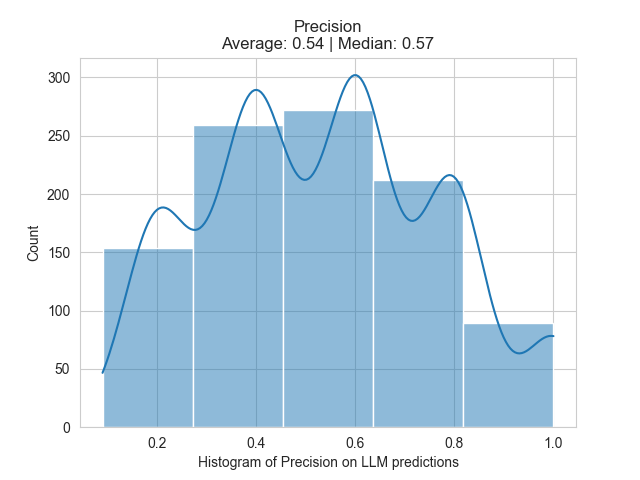
\includegraphics[width=1\linewidth]{doc//report//assets/llm-precision.png}
    \caption{Precision of LLM Responses}
    \label{fig:llm-precision}
\end{figure}


\subsubsection{Recall}
The recall of LLM responses on 1111 test cases is shown in Figure \ref{fig:llm-recall}. It is no surprise that we observed a rather low and unbalanced recall distribution. This is due to a hard cut-off of false negative counts and the limit of the number of movies that can be generated by the LLM.

\begin{figure}
    \centering
    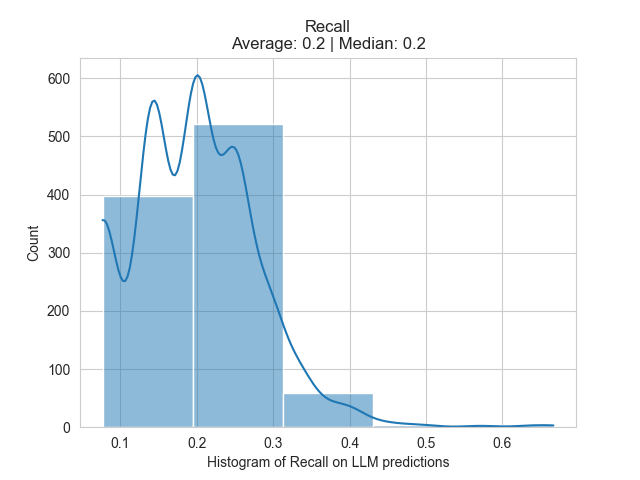
\includegraphics[width=1\linewidth]{doc//report//assets/llm-recall.png}
    \caption{Recall of LLM Responses}
    \label{fig:llm-recall}
\end{figure}

\subsection{Cluster Response}
\subsubsection{Precision}
The comparison of precision of two clustering methods are shown in Figure \ref{fig:cluster-precision}. Both models show a relatively lower score of precision. For K-means algorithm, this because of the cluster size and our ranking mechanism. We only have 286 clusters and we rank the movies based on their popularity. This can cause precision to drop because potential movies in the same cluster might be replaced by other movies that are in the same cluster but receive higher reputation. For TF-IDF algorithm, this is because depending only on plot feature of the movie is not entirely reliable. Because the tune and wording preferences of movie plot can have an impact on the similarity between movies.

\begin{figure}
    \centering
    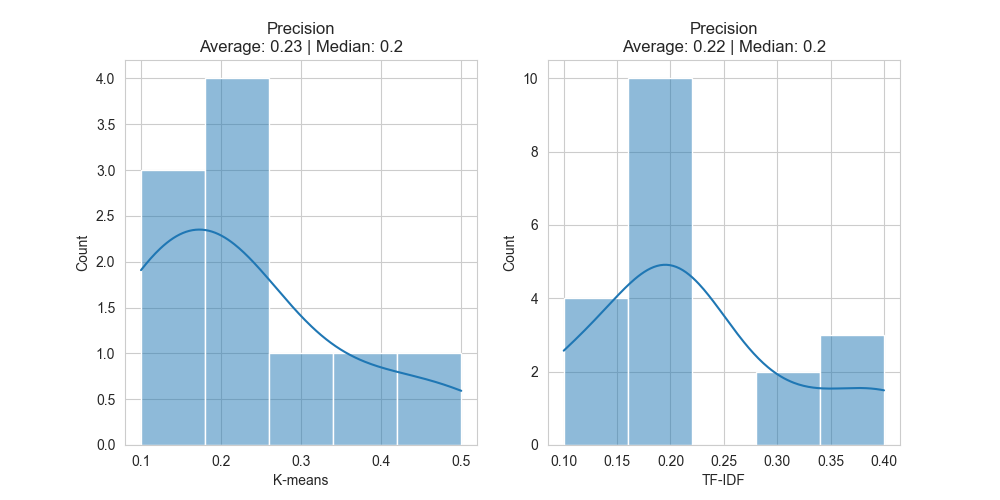
\includegraphics[width=1\linewidth]{doc//report//assets/precision-comparison.png}
    \caption{Precision of Cluster Responses}
    \label{fig:cluster-precision}
\end{figure}


\subsubsection{Recall}
The comparison of recall of two clustering methods are shown in Figure \ref{fig:cluster-recall}. Both methods show an higher recall than LLM responses. This is because the hard cut-off in False Negative counts is lifted. There is no significant difference in clustering results.

\begin{figure}
    \centering
    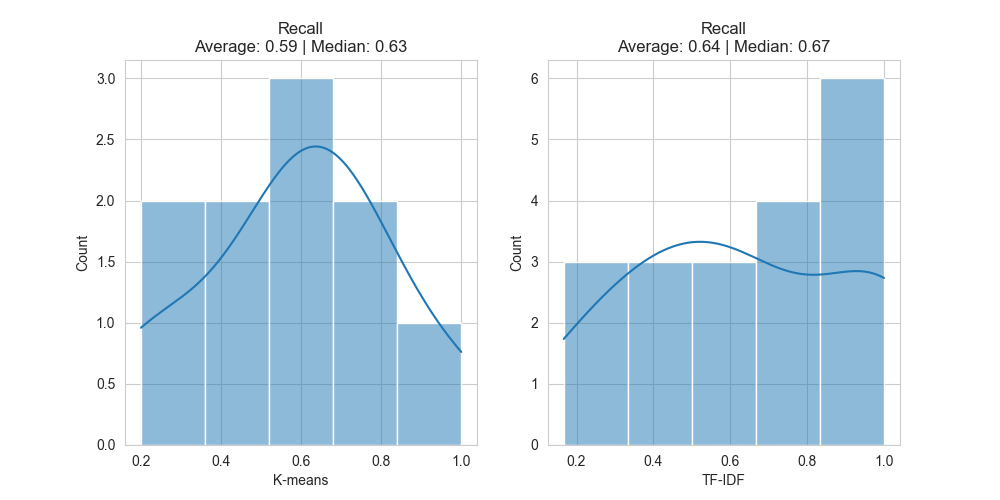
\includegraphics[width=1\linewidth]{doc//report//assets/recall-comparison.png}
    \caption{Recall of Cluster Responses}
    \label{fig:cluster-recall}
\end{figure}

\section{Conclusion}

In our research, we have developed an innovative movie search and recommendation system that leverages Large Language Models (LLMs) to enhance the precision and relevance of movie recommendations and queries. By focusing on semantic understanding of user queries through LLMs, our system addresses the challenge of the overwhelming choice users face on streaming platforms, significantly reducing the time users spend browsing for movies.

Our motivation is that we believe incorporating LLMs improves the interaction between users and the system, allowing for a more intuitive and personalized search experience. Users can query movies based on nuanced preferences and receive recommendations that better align with their desires, not just based on metadata but also on thematic elements, narrative styles, or emotional tones. This represents a considerable shift from traditional search mechanisms that rely heavily on metadata and often fail to fully capture the individual user's needs.

Our results, not only shows a high level of usefulness both functionally and user-friendly, but it has also been tested by the self built dataset. We realized the lack of performance and evaluation metrics, ground truth and dataset in this field and proposed tag-based and sequel-based ways to construct ground truth of movie recommendation.

Overall, the implementation of our LLM-driven movie search and recommendation system represents a significant advancement in how users interact with movie database, making the process more efficient, accurate, and user-friendly. This could potentially set a new standard for content discovery in streaming platforms, thereby enhancing user satisfaction and engagement with digital media services.

% In this project, our group designed an LLM-based method and prompt the LLM as a “judge” to evaluate the performance and accuracy of our movie recommendation system. Specifically, we set a task to the LLM and requested an evaluation of our movie recommendation system's accuracy in matching movies to specific queries. The task involved scoring each recommended movie based on how well it aligned with the input queries, using a predefined scale: 2 for a “good match”, 1 for a “partial match”, and 0 for a “not much of a match”. The score is called “relevance score”. This method aimed to assess the system's effectiveness in understanding and responding to diverse movie-related queries with relevant recommendations. Below is the case study for the Evaluation system, for the Table~\ref{tab:movie_queries} , 5 movies and 3 quires (randomly selected by our group) are listed, and the relevance score matrix from the LLM is shown in Table~\ref{tab:query_frequency}:
% \begin{table}[h!]
% \centering
% \caption{The Movies and Queries Used in the Evaluation System Case Study}
% \begin{tabular}{|c|l|l|}
% \hline
% \textbf{\#} & \textbf{Movie}                 & \textbf{Query}                       \\ \hline
% 1           & The Shawshank Redemption       & A man run across United States       \\ \hline
% 2           & Forrest Gump                   & Brave People                         \\ \hline
% 3           & Avatar                         & Car                                  \\ \hline
% 4           & The Godfather                  &                                      \\ \hline
% 5           & Saw                            &                                      \\ \hline
% \end{tabular}
% \label{tab:movie_queries}
% \end{table}
% \begin{table}[h!]
% \centering
% \caption{The Relevance Score Matrix of the Evaluation System Case Study}
% \begin{tabular}{|l|c|c|c|}
% \hline
% \textbf{Movie}              & \makecell{\textbf{A man run} \\ \textbf{across United States}} & \textbf{Brave People} & \textbf{Car} \\ \hline
% The Shawshank Redemption    & 0                                       & 1                     & 0            \\ \hline
% Forrest Gump                & 2                                       & 1                     & 0            \\ \hline
% Avatar                      & 0                                       & 1                     & 0            \\ \hline
% The Godfather               & 0                                       & 1                     & 1            \\ \hline
% Saw                         & 0                                       & 1                     & 0            \\ \hline
% \end{tabular}
% \label{tab:query_frequency}
% \end{table}

% Note that although the score matrix only displays the “relevance score”, in fact, the LLM provided a short paragraph to briefly explain why the score was assigned to each movie-query combination. The full output is presented in the Appendix of this report.

% The relevance score matrix shows the relevance between each query and each movie.  For example, if the query is “A man run across the United States”, the score of the movie “Forrest Gump” is 2, which means the query and movie are a good match, indicating our system made a good recommendation. On the other hand, the score of the movie “The Shawshank Redemption” is 0, which means the movie and query are not match, and indicating our system made a bad recommendation.

% Based on the knowledge of these movies, our group believes the evaluation score for each case is accurate and promising. In this case, the evaluation system is reliable.  


%User interface Sectio

% references section
\bibliographystyle{IEEEtran}
\bibliography{IEEEabrv, proposal-ref}

% \section{Appendix}
% \subsection{Timetable and Work Distribution for the Project}
% This project is undertaken by a team comprising three members: Micah Harlan, Baiyi Zhang, and Jianger Yu. Each member is tasked with leveraging their specific expertise to contribute significantly to the project's completion. The project is organized into five distinct sections. As of March 19, 2024, the Data and Storage components, as well as the Application Programming Interface (API), have been successfully implemented. The forthcoming stages—namely the Large Language Model (LLM) and the Recommendation System—are scheduled for completion by April 9, 2024. The final phase, focusing on the User Interface (UI) development, is projected to be completed by May 7, 2024, thereby finalizing the application.

% \subsection{Full Output of the LLM for the Evaluation System Case Study}
% The complete output of the Large Language Model (LLM) for the evaluation system case study is provided in the supplementary material section at the conclusion of this document.

% \subsection{Sample Result of Query API}
% The sample result of the query API is provided in the supplementary material section at the conclusion of this document.

% \subsection{Sample Result of LLM Summary}
% The sample result of the summary by the LLM is provided in the supplementary material section at the conclusion of this document.

% \subsection{Progress Report}
% In this progress report, we're detailing the contributions of each team member up to the current checkpoint.

% Baiyi Zhang had completed the Design Overview and System Architecture, integrated the API into our project, and developed tasks for Large Language Models as of Checkpoint 1. As of Checkpoint 2, he finished implementing server using FastAPI to interact with the database. He also implemented proof-of-concept task of utilizing open source large language model for query result summarizing.

% During Checkpoint 1 Micah Harlan focused on the database aspect, designing the schema, creating the database itself, and handling dataset pre-processing. In Checkpoint 2, Micah leveraged CSS, HTML, and JavaScript to create the user interface that a user can search and view results. He also connected the LLM to the front end of the project so the users can search and communicate with the back end.

% During checkpoint 1, Jianger Yu has set up the large language model (LLM) for this project and ran the test for movie description generation. During checkpoint 2, Jianger Yu had developed the evaluation methods for the movie recommendation system, and used the LLM to perform a case study.
\end{document}